%% Generated by Sphinx.
\def\sphinxdocclass{report}
\documentclass[a4paper,12pt,english]{sphinxmanual}
\ifdefined\pdfpxdimen
   \let\sphinxpxdimen\pdfpxdimen\else\newdimen\sphinxpxdimen
\fi \sphinxpxdimen=.75bp\relax

\PassOptionsToPackage{warn}{textcomp}
\usepackage[utf8]{inputenc}
\ifdefined\DeclareUnicodeCharacter
% support both utf8 and utf8x syntaxes
\edef\sphinxdqmaybe{\ifdefined\DeclareUnicodeCharacterAsOptional\string"\fi}
  \DeclareUnicodeCharacter{\sphinxdqmaybe00A0}{\nobreakspace}
  \DeclareUnicodeCharacter{\sphinxdqmaybe2500}{\sphinxunichar{2500}}
  \DeclareUnicodeCharacter{\sphinxdqmaybe2502}{\sphinxunichar{2502}}
  \DeclareUnicodeCharacter{\sphinxdqmaybe2514}{\sphinxunichar{2514}}
  \DeclareUnicodeCharacter{\sphinxdqmaybe251C}{\sphinxunichar{251C}}
  \DeclareUnicodeCharacter{\sphinxdqmaybe2572}{\textbackslash}
\fi
\usepackage{cmap}
\usepackage[T1]{fontenc}
\usepackage{amsmath,amssymb,amstext}
\usepackage{babel}
\usepackage{times}
\usepackage[Sonny]{fncychap}
\ChNameVar{\Large\normalfont\sffamily}
\ChTitleVar{\Large\normalfont\sffamily}
\usepackage{sphinx}
\usepackage{pdfpages}

\fvset{fontsize=\small}
\usepackage{geometry}

% Include hyperref last.
\usepackage{hyperref}
% Fix anchor placement for figures with captions.
\usepackage{hypcap}% it must be loaded after hyperref.
% Set up styles of URL: it should be placed after hyperref.
\urlstyle{same}

\addto\captionsenglish{\renewcommand{\figurename}{Fig.\@ }}
\makeatletter
\def\fnum@figure{\figurename\thefigure{}}
\makeatother
\addto\captionsenglish{\renewcommand{\tablename}{Table }}
\makeatletter
\def\fnum@table{\tablename\thetable{}}
\makeatother
\addto\captionsenglish{\renewcommand{\literalblockname}{Listing}}

\addto\captionsenglish{\renewcommand{\literalblockcontinuedname}{continued from previous page}}
\addto\captionsenglish{\renewcommand{\literalblockcontinuesname}{continues on next page}}
\addto\captionsenglish{\renewcommand{\sphinxnonalphabeticalgroupname}{Non-alphabetical}}
\addto\captionsenglish{\renewcommand{\sphinxsymbolsname}{Symbols}}
\addto\captionsenglish{\renewcommand{\sphinxnumbersname}{Numbers}}

\addto\extrasenglish{\def\pageautorefname{page}}

\setcounter{tocdepth}{1}



\title{eyes17 Documentation}
\date{Feb 28, 2020}
\release{1.0}
\author{GK}
\newcommand{\sphinxlogo}{\vbox{}}
\renewcommand{\releasename}{Release}
\makeindex
\begin{document}

\ifdefined\shorthandoff
  \ifnum\catcode`\=\string=\active\shorthandoff{=}\fi
  \ifnum\catcode`\"=\active\shorthandoff{"}\fi
\fi

\pagestyle{empty}
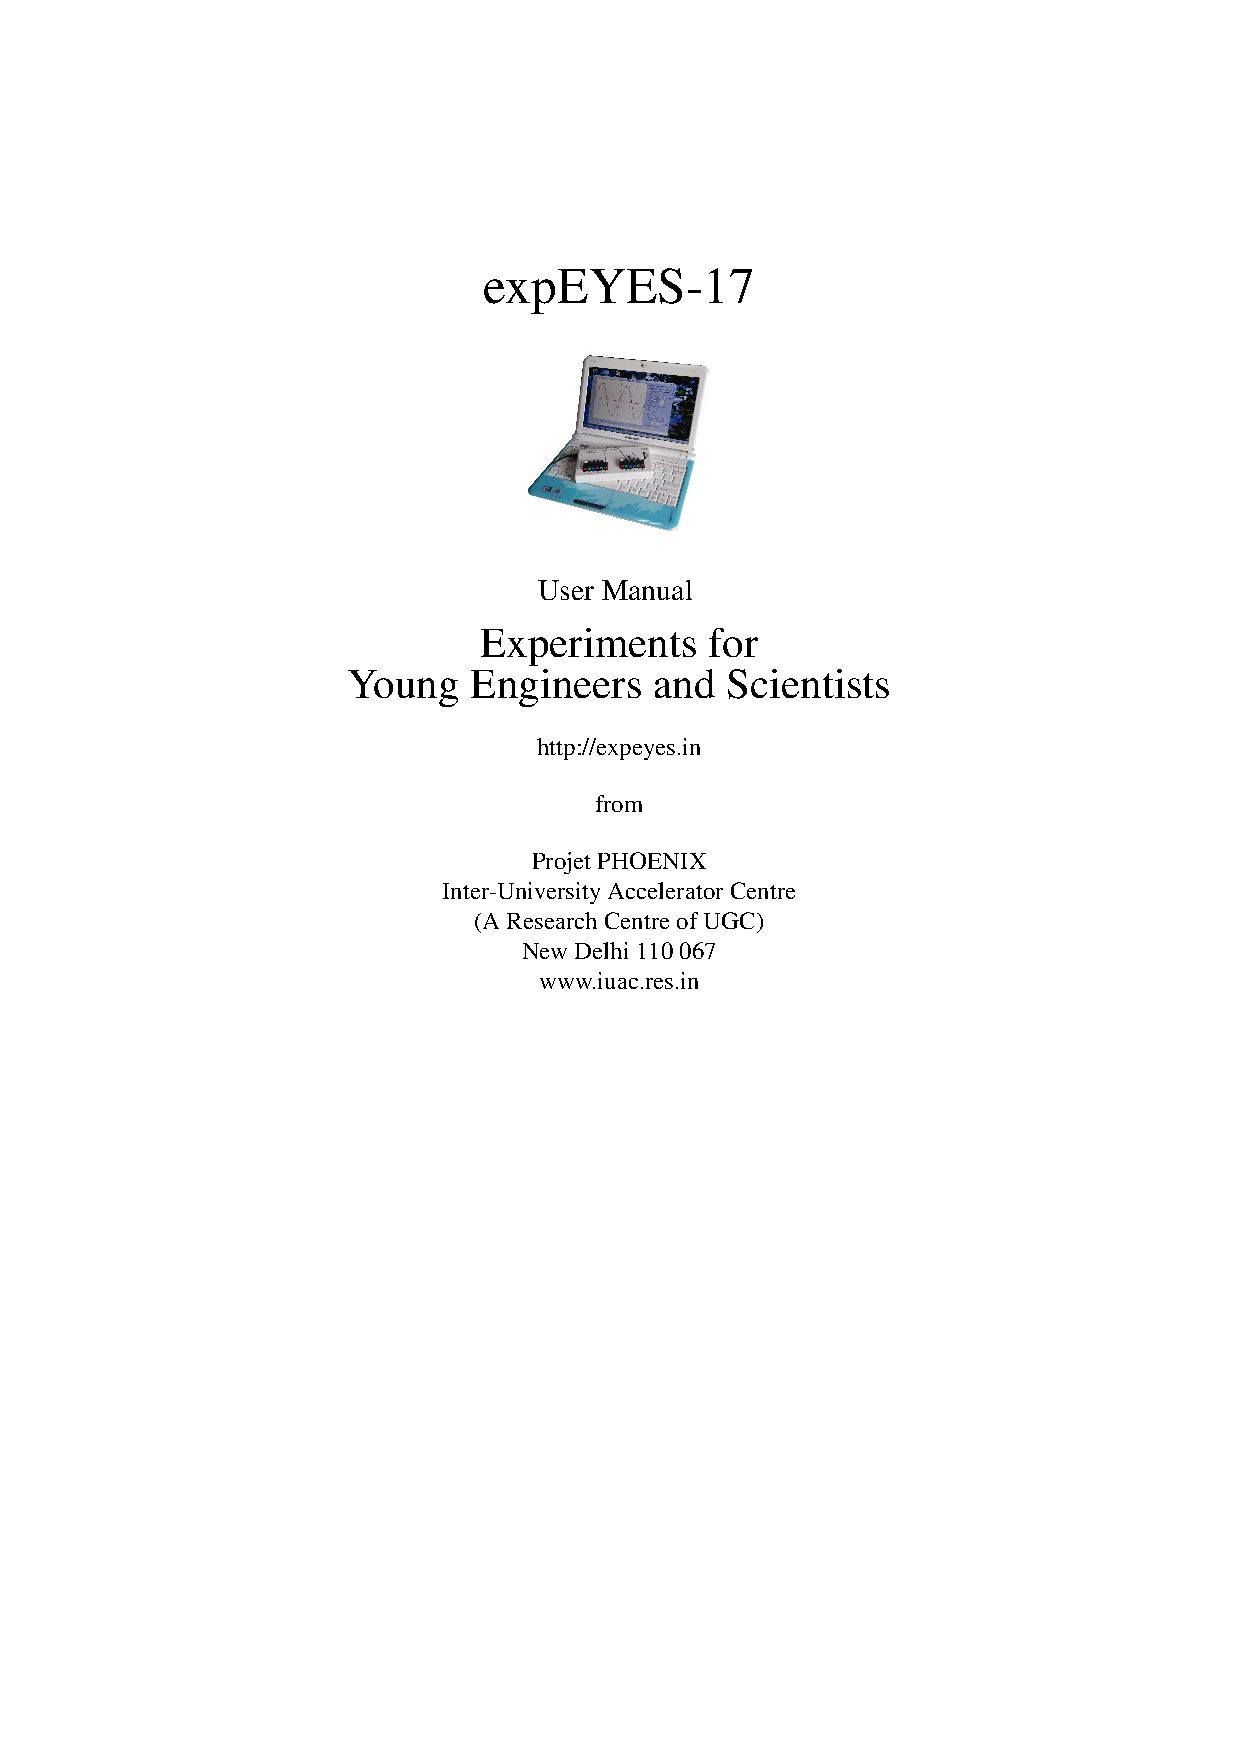
\includepdf{coverpage.pdf}
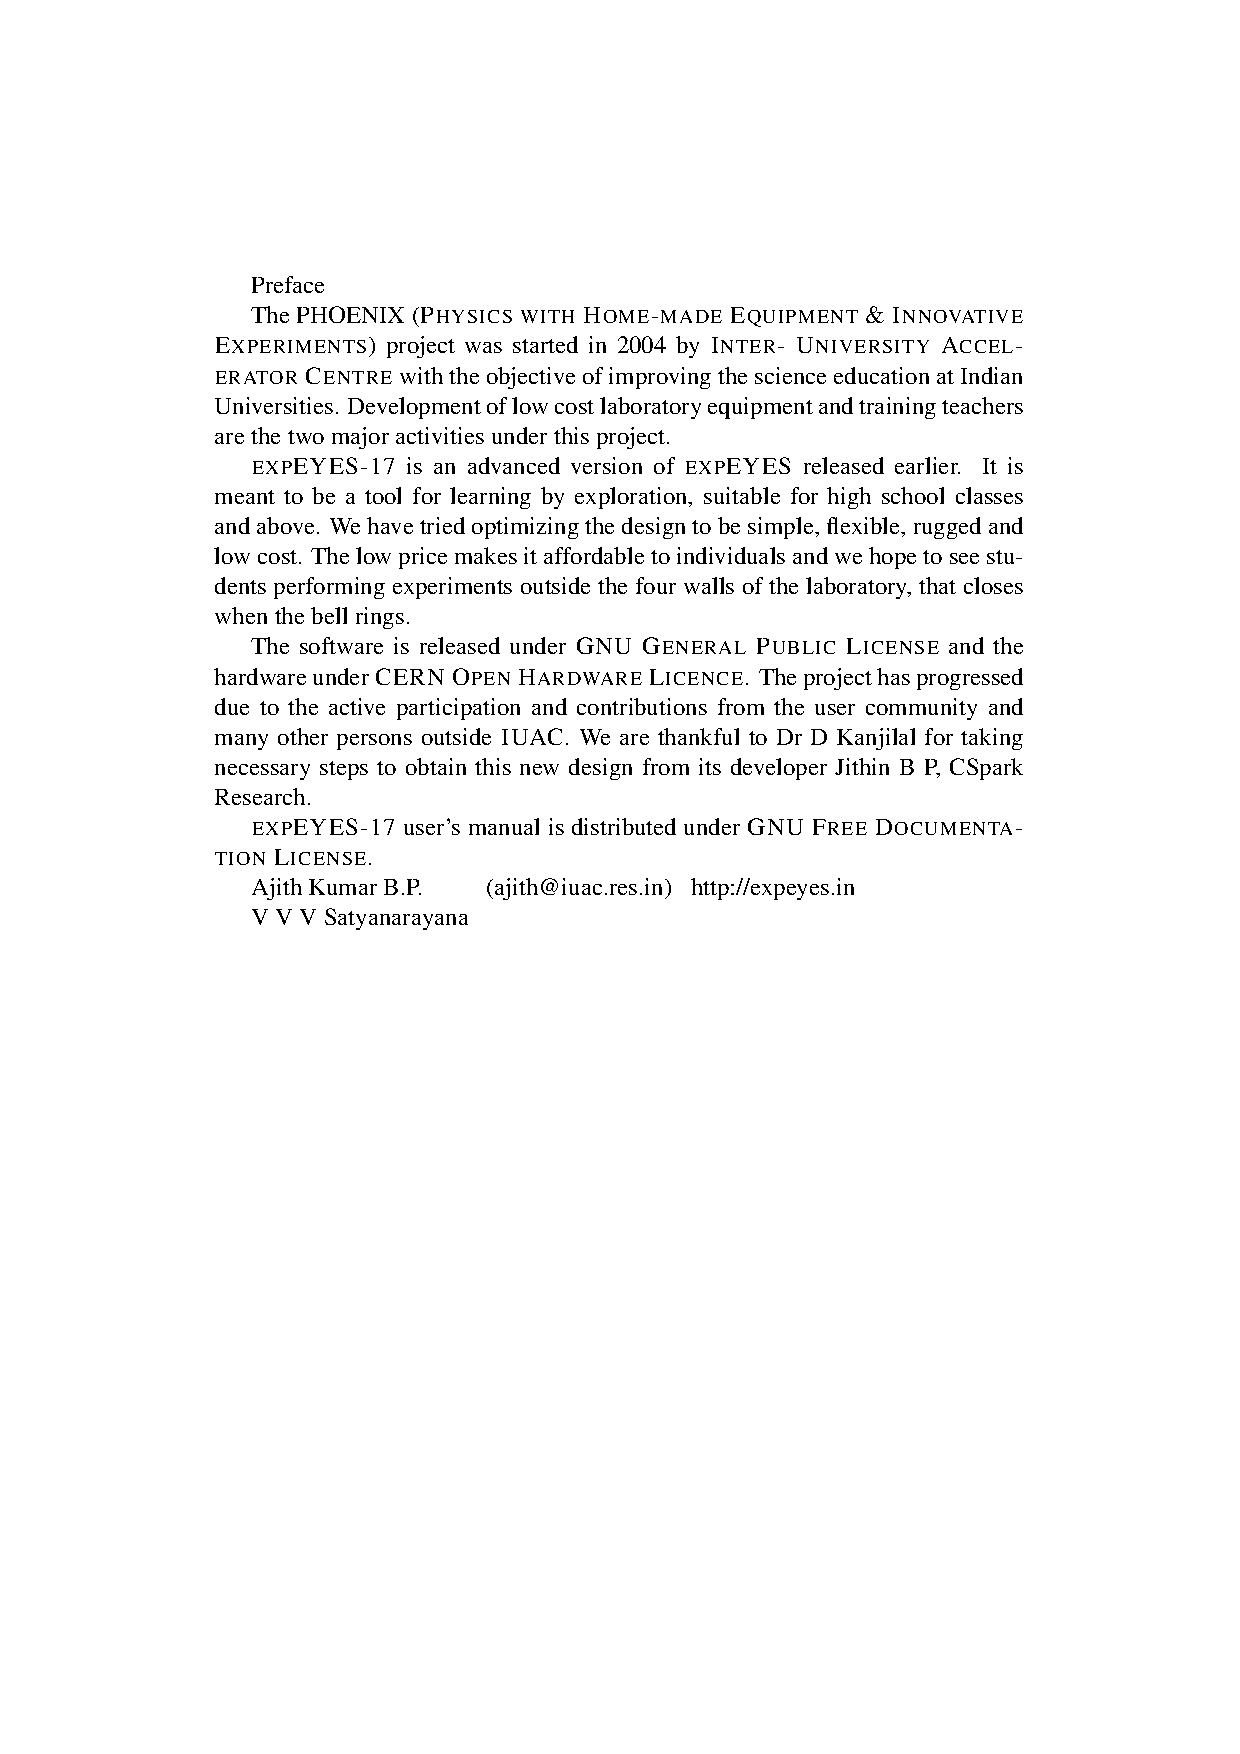
\includepdf{preface.pdf}
\pagestyle{plain}
\sphinxtableofcontents
\pagestyle{normal}
\phantomsection\label{\detokenize{index::doc}}



\chapter{Introduction}
\label{\detokenize{1.1:introduction}}\label{\detokenize{1.1::doc}}
Science is the study of the physical world by systematic observations
and experiments. Proper science education is essential for cultivating a
society where reasoning and logical thinking prevails and not
superstition and irrational beliefs. Science education is also essential
for training enough technicians, engineers and scientists for the
economy of the modern world. It is widely accepted that personal
experience in the form of experiments and observations, either carried
out by students or performed as demonstrations by teachers, are
essential to the pedagogy of science. However, almost everywhere science
is mostly taught from the text books without giving importance to
experiments, partly due to lack of equipment. As a result, most of the
students fail to correlate their classroom experience to problems
encountered in daily life. To some extent this can be corrected by
learning science based on exploration and experimenting.

The advent of personal computers and their easy availability has opened
up a new path for making laboratory equipment. Addition of some hardware
to an ordinary computer can convert it in to a science laboratory.
Performing quick measurements with good accuracy enables one to study a
wide range of phenomena. Science experiments generally involve
measuring/controlling physical parameters like temperature, pressure,
velocity, acceleration, force, voltage, current etc. If the measured
physical property is changing rapidly, the measurements need to be
automated and a computer becomes a useful tool. For example,
understanding the variation of AC mains voltage with time requires
measuring it after every millisecond.

The ability to perform experiments with reasonable accuracy also opens
up the possibility of research oriented science education. Students can
compare the experimental data with mathematical models and examine the
fundamental laws governing various phenomena. Research scientists do the
same with highly sophisticated equipment. The expEYES ( expEriments for
Young Engineers \& Scientists) kit is designed to support a wide range of
experiments, from school to post graduate level. It also acts as a test
equipment for electronics engineers and hobbyists. The simple and open
architecture of expEYES allows the users to \sphinxstyleemphasis{develop new experiments,
without getting into the details of electronics or computer
programming}. This User’s manual describes \sphinxstyleemphasis{expEYES-17} along with
several experiments, there is also a Programmer’s manual available.


\chapter{The equipment}
\label{\detokenize{1.2:the-equipment}}\label{\detokenize{1.2::doc}}
ExpEYES-17 is interfaced and powered by the USB port of the computer,
and it is programmable in Python. It can function as a low frequency
oscilloscope, function generator, programmable voltage source, frequency
counter and data logger. For connecting external signals, it has two
spring loaded terminals blocks, one for output signals and another for
inputs, as shown in figure {\hyperref[\detokenize{1.2:fig:The-ExpEYES-toppanel}]{\emph{1.1}}}. The
software can monitor and control the voltages at these terminals. In
order to measure other parameters (like temperature, pressure etc.), we
need to convert them in to electrical signals by using appropriate
sensor elements. The accuracy of the voltage measurements is decided by
the stability of the 3.3V reference used, it is 50ppm per degree
celcius. The gain and offset errors are eliminated by initial
calibration, using a 16bit ADC. Even though our primary objective is to
do experiments, you are advised to read through the brief description of
the equipment given below. The device can be also used as a test
equipment for electrical and electronics engineering experiments.

\sphinxstyleemphasis{IMPORTANT :}

\sphinxstyleemphasis{The external voltages connected to ExpEYES17 must be within the allowed
limits. Inputs A1 and A2 must be within \(\pm\)16 volts range and Inputs IN1
and IN2 must be in 0 to 3.3V range. Exceeding these limits may result in
damage to the equipment. To measure higher voltages, scale them down
using resistive potential divider networks.}

\begin{figure}[htbp]
\centering

\noindent\sphinxincludegraphics[width=500\sphinxpxdimen]{{eyes17-panel}.pdf}
\end{figure}

Figure 1.1 The ExpEYES17 top panel showing the external connections.


\section{External connections}
\label{\detokenize{1.2:external-connections}}
The functions of the external connections briefly explained below. All
the black coulored terminals are at ground potential, all other voltages
are measured with respect to it.


\subsection{Outputs:}
\label{\detokenize{1.2:outputs}}

\subsubsection{Constant Current Source (CCS) :}
\label{\detokenize{1.2:constant-current-source-ccs}}
The constant current source can be switched ON and OFF under software
control. The nominal value is 1.1 mA but may vary from unit to unit, due
to component tolerances. To measure the exact value, connect an ammeter
from CCS to GND. Another method is to connect a known resistance (\textasciitilde{}1k)
and measure the voltage drop across it. The load resistor should be less
than 3k for this current source.


\subsubsection{Programmable Voltage (PV1) :}
\label{\detokenize{1.2:programmable-voltage-pv1}}
Can be set, from software, to any value in the -5V to +5V range. The
resolution is 12 bits, implies a minimum voltage step of around 2.5
millivolts.


\subsubsection{Programmable Voltage (PV2) :}
\label{\detokenize{1.2:programmable-voltage-pv2}}
Can be set, from software, to any value in the -3.3V to +3.3V range. The
resolution is 12 bits.


\subsubsection{Square Wave SQ1:}
\label{\detokenize{1.2:square-wave-sq1}}
Output swings from 0 to 5 volts and frequency can be varied 4Hz to
100kHz. All intermediate values of frequency are not possible. The duty
cycle of the output is programmable. Setting frequency to 0Hz will make
the output HIGH and setting it to  - 1 will make it LOW, in both cases
the wave generation is disabled. SQR1 output has a \(100~\Omega\) \sphinxstylestrong{series
resistor} inside so that it can drive LEDs directly.


\subsubsection{Square Wave SQ2:}
\label{\detokenize{1.2:square-wave-sq2}}
Output swings from 0 to 5 volts and frequency can be varied 4Hz to
100kHz. All intermediate values of frequency are not possible. The duty
cycle of the output is programmable. SQR2 is not available when WG is
active.


\subsubsection{Digital Output (OD1) :}
\label{\detokenize{1.2:digital-output-od1}}
The voltage at OD1 can be set to 0 or 5 volts, using software.


\subsubsection{Sine/Triangular Wave WG:}
\label{\detokenize{1.2:sine-triangular-wave-wg}}
Frequency can be varied from 5Hz to 5kHz. The peak value of the
amplitude can be set to 3 volts, 1.0 volt or 80 mV. Shape of the output
waveform is programmable. Using the GUI sine or triangular can be
selected. WG bar is inverted WG.


\subsection{Inputs:}
\label{\detokenize{1.2:inputs}}

\subsubsection{Capacitance meter IN1:}
\label{\detokenize{1.2:capacitance-meter-in1}}
Capacitance connected between IN1 and Ground can be measured. It works
better for lower capacitance values, upto 10 nanoFarads, results may not
be very accurate beyond that.


\subsubsection{Frequency Counter IN2:}
\label{\detokenize{1.2:frequency-counter-in2}}
Capable of measuring frequencies upto several MHz.


\subsubsection{Resistive Sensor Input (SEN):}
\label{\detokenize{1.2:resistive-sensor-input-sen}}
This is mainly meant for sensors like Light Dependent Resistor,
Thermistor, Photo-transistor etc. SEN is internally connected to 3.3
volts through a 5.1k\(\Omega\) resistor.


\subsubsection{\protect\(\pm16\ V\protect\) Analog Inputs, A1 \& A2:}
\label{\detokenize{1.2:pm16-v-analog-inputs-a1-a2}}
Can measure voltage within the \(\pm\)16 volts range. The input voltage range
can be selected from .5V to 16V fullscale. Voltage at these terminals
can be displayed as a function of time, giving the functionality of a
low frequency oscilloscope. The maximum sampling rate is 1 Msps
/channel. Both have an input impedance of 1M\(\Omega\) .


\subsubsection{\protect\(\pm3.3\ V\protect\) Analog Input A3:}
\label{\detokenize{1.2:pm3-3-v-analog-input-a3}}
Can measure voltage within the \(\pm\)3.3 volts range. The input can be
amplified by connecting a resistor from Rg to Ground, gain
=1 + (Rg)/(10000). This enables displaying very small amplitude signals.
The input impedance of A3 is 10M\(\Omega\).


\subsubsection{Microphone input MIC:}
\label{\detokenize{1.2:microphone-input-mic}}
A condenser microphone can be connected to this terminal and the output
can be captured.


\subsection{I2C Sensor Interface:}
\label{\detokenize{1.2:i2c-sensor-interface}}
The four connections (+5V, Ground, SCL and SDA) of the 8 terminal berg
strip supports I2C sensors. The software is capable of recognizing a
large number of commercially available I2C sensors.


\subsection{\protect\(\pm\ 6\ V/10\ mA\protect\) Power supply:}
\label{\detokenize{1.2:pm-6-v-10-ma-power-supply}}
The VR+ and VR- are regulated power outputs. They can supply very little
current, but good enough to power an Op-Amp.


\section{1.2.2 Accessory Set}
\label{\detokenize{1.2:accessory-set}}
Some accessories are provided with expEYES.
\begin{itemize}
\item {} 
Pieces of wires, with pin and with crocodile clip.

\item {} 
Condenser microphone with leads.

\item {} 
Inductor Coil (2) : 44SWG wire on 1cm dia bobbin. Around 3000 Turns
(some may have more turns). These coils can be used for studying
inductance, electromagnetic induction etc.

\item {} 
Piezo Electric Discs (2) : Resonant frequency is around 3500 Hz. Can
be energized by WG output or SQR1. Discs are enclosed in a plastic
shell that forms a cavity, that enhances the amplitude of sound
produced.

\item {} 
DC Motor : Should be powered by a DC voltage less than 3 volts.

\item {} 
Permanent Magnets : (a) 10mm dia \& length (b) 5 mm dia \& 10 mm length (c)
Button size magnets(2)

\item {} 
5mm LEDS : RED, BLUE, GREEN, WHITE

\item {} 
Capacitors : 100pF, 0.1uF , 1 uF \& 22uF

\item {} 
Inductor : 10 mH / 20\(\Omega\),

\item {} 
Resistors : 560\(\Omega\), 1k\(\Omega\), 2.2k\(\Omega\) , 10k\(\Omega\) , 51k\(\Omega\) and 100 k\(\Omega\)

\item {} 
LDR

\item {} 
Two silicon diodes (1N4148) and one 3.3 volts zener diode

\item {} 
NPN Transistor( 2N2222)

\end{itemize}


\chapter{Software Installation}
\label{\detokenize{1.3:software-installation}}\label{\detokenize{1.3::doc}}
ExpEYES can run on any computer having a Python Interpreter and required
modules. The USB interface is handled by a device driver program that
presents the USB port as a Serial port to the Python programs. The
communication the expEYES is done using a library written in Python.
Programs with GUI have been written for many experiments. Eyes17
software require the following packages
\begin{itemize}
\item {} 
python-serial

\item {} 
python-numpy

\item {} 
python-scipy

\item {} 
python-qt4

\item {} 
python-pyqtgraph

\end{itemize}


\section{Any GNU/Linux distributions}
\label{\detokenize{1.3:any-gnu-linux-distributions}}
Download \sphinxstylestrong{eyes17-x.x.x.zip} (the latest version) from
\sphinxstylestrong{http://expeyes.in} and upzip it, and change to the newly created
folder. Issue the command
\begin{quote}

\$ sudo sh postinst       \# set user write permission

\$ python main.py
\end{quote}

You will get error messages for any missing packages that are required
for expeyes. Install them one by one and try again. Python programs
required for several experiments are in the same directory, they are
called by ’main.py’.


\section{Debian or Ubuntu GNU/Linux distributions}
\label{\detokenize{1.3:debian-or-ubuntu-gnu-linux-distributions}}
Download \sphinxstylestrong{eyes17-x.x.x.deb} ( the latest version) from the software
section of \sphinxstylestrong{http://expeyes.in} and install it using the command;
\begin{quote}

\$ sudo gdebi eyes17-x.x.x.deb
\end{quote}

while connected to Internet

The package ’eyes17’ (later than version 3) does not depend on the
earlier versions of ExpEYES, like expeyes junior. During installation
gdebi will automatically dowload and install all the required packages.


\section{The expEYES Live CD / USB pendrive}
\label{\detokenize{1.3:the-expeyes-live-cd-usb-pendrive}}
The ISO image containing support for eyes17 can be downloaded from HERE.
Make a DVD or USB memory stick bootable using this ISO image (Download
rufus from \sphinxurl{https://rufus.akeo.ie} to do this under MSWindows)

Switch off the PC and insert the liveCD/Pendrive and switch it on. Enter
the BIOS while booting, make the CDdrive/USB hard disk as the first boot
device. A desktop will appear and you can start expEYES-17 from the menu
\sphinxstylestrong{Applications-\textgreater{}Education}-\textgreater{}ExpEYES-17. You can also start it from a
Terminal using the command:
\begin{quote}

\$ python /usr/share/expeyes/eyes17/main.py
\end{quote}


\section{On MSWindows}
\label{\detokenize{1.3:on-mswindows}}
The first thing to do is to install the driver software for the USB to
serial converter IC MCP2200, available on Microchip website (also given
on expeyes website). After installing this the device will appear as a
COM port, that can be verified from the device manager of MSWindows.
After this there are two options.

A zip file containing all the necessary things for ExpEYES is available
on the website, named eyes17win.zip. Unzip this file and run main.py
from that. By using this method you will not able to write your own
Python code to access expeyes, for that you need to install the
following
\begin{enumerate}
\def\theenumi{\arabic{enumi}}
\def\labelenumi{\theenumi .}
\makeatletter\def\p@enumii{\p@enumi \theenumi .}\makeatother
\item {} 
Python-2.x version

\item {} 
python-serial

\item {} 
python-qt4

\item {} 
python-pyqtgraph,

\item {} 
python-numpy

\item {} 
python-scipy

\end{enumerate}

Download the eyes17-x.x.x.zip ( take latest version) from the website.
Unzipping the files will create a directory \sphinxstylestrong{named eyes17}, run
\sphinxstylestrong{main.py} from that.


\chapter{The main GUI program}
\label{\detokenize{1.4:the-main-gui-program}}\label{\detokenize{1.4::doc}}
Start Applications-\textgreater{}Education-\textgreater{}ExpEYES-17 from the menu. A four channel
oscilloscope screen with several extra features will open as shown in
figure {\hyperref[\detokenize{1.4:the-scope17-screen}]{\sphinxcrossref{\DUrole{std,std-ref}{The scope17 screen showing two traces}}}}. Various experiments can be
selected from the menu.

\begin{figure}[htbp]
\centering
\capstart

\noindent\sphinxincludegraphics{{scope17}.pdf}
\caption{The scope17 screen showing two traces}\label{\detokenize{1.4:id1}}\label{\detokenize{1.4:the-scope17-screen}}\end{figure}

The main window looks like a low frequency four channel oscilloscope,
with some extra features, on the right side panel. Applications for
various experiments can be selected from the pulldown menu. A brief
description of the oscilloscope program is given below.
\begin{itemize}
\item {} 
Any of the four inputs (A1, A2, A3 or MIC) can be enabled using the
corresponding checkbox. The input range can be selected by clicking
on the menubutton on the right side of the checkbox. Select the
desired input range from the popup menu.

\item {} 
There is another checkbox, to enable mathematical fitting of the data
using V = V0sin(2\(\pi\)ft + \(\theta\)) + C to show the amplitude and
frequency.

\item {} 
The horizontal scale (time base) can be changed by a slider, from .5
mS fullscale to 500 mS full scale.

\item {} 
The Checkbutton \sphinxstylestrong{Freeze}, allows to pause and resume the
oscilloscope operation.

\item {} 
The Trigger level can be set by a slider, and there is a menubutton
to select the trigger source.

\item {} 
To save the traces to a file, edit the filename and click on the
\sphinxstylestrong{SaveTo} button.

\item {} 
Clicking on \sphinxstylestrong{FFT} shows the frequency spectrum of all the eneabled
channels, appears on popup windows.

\end{itemize}

In addition to the Oscilloscope, there are several measurement/control
options available on the GUI, they are explained below.
\begin{itemize}
\item {} 
If selected, the voltages at the inputs A1, A2 and A3 are sampled
every second and displayed.

\item {} 
The resistance connected between SEN and Ground is measured and
displayed every second.

\item {} 
Clicking \sphinxstylestrong{Capacitance on IN1}, measures the value of the capacitor
connected between IN1 and GND.

\item {} 
Clicking \sphinxstylestrong{Frequency on IN2}, measures the frequency of an external
digital (TTL standard) pulse connected to IN2

\item {} 
The shape of the waveform can be selected using the menubutton,
default shape is sine. It can be changed to triangular. When the
square wave option is selected, the output is shifted to SQ2. You
cannot have sine/triangular and SQ2 at the same time.

\item {} 
Frequency of the Waveform generator WG can be set using the slider or
the text entry window. The two input methods follow each other,
changing the slider will change the text field and entering data
using text field will set the slider to that value. The frequency
will be set to the nearest possible value and it will be displayed in
the message window at the bottom. The amplitude of WG output can be
set to 3 volts, 1 volt or 80 mV.

\item {} 
SQ1 can be set using the same method as explained above. The duty
cycle can be set between 1\% to 99\%, default is 50\%.

\item {} 
The programmable volages PV1 and PV2 are also set in a similar
manner.

\item {} 
Checkbuttons are provided to control OD1 and CCS.

\end{itemize}


\chapter{Getting Familiar with ExpEYES17}
\label{\detokenize{1.5:getting-familiar-with-expeyes17}}\label{\detokenize{1.5::doc}}
Before proceeding with the experiments, let us do some simple exercises
to become familiar with expEYES-17. Connect the device a USB port and
start the ExpEYES-17 program from the menu ’Applications-\textgreater{}Education’.
Enable the ’Popup Help’ option and select the first few items from the
school menu.

The following chapters are organized according to the pulldown menus of
the eyes17 program, each chapter containing the experiments under the
corresponding menu; like School level, Eelectronics, Eelectrical etc. To
perform the expeiment, select it from the menu. Online help is available
for every experiment, making this manual almost redundant.

The screen shots given in this document are not from the GUI program,
because the black background images are difficult to print. The plots
are generated by separate code.


\chapter{School Level Experiments}
\label{\detokenize{index:school-level-experiments}}
This chapter will discuss the experiments and demonstrations without
much data analysis, experiments given in the menu SchoolExpts. Simple
tasks like measuring voltage, resistance, capacitance etc. will be done
followed by resistances changing with temperature or light. The concept
of Alternating Current is introduced by plotting the voltage as a
function of time. Generating and digitizing sound will be covered. When
an experiment is selected, the corresponding help window will popup, if
enabled.


\section{Measuring Voltage}
\label{\detokenize{2.1:measuring-voltage}}\label{\detokenize{2.1::doc}}
\sphinxstylestrong{Objective}

Learn to measure voltage using expEYES and get some idea about the
concept of Electrical Ground. A dry-cell and two wires are required.

\noindent\sphinxincludegraphics[width=300\sphinxpxdimen]{{measure-dc}.pdf}

\sphinxstylestrong{Procedure}
\begin{itemize}
\item {} 
Observe the voltage at A1 displayed.

\item {} 
Repeat by reversing the cell connections.

\end{itemize}

\sphinxstylestrong{Discussion}

Voltages measured value is +1.5 volts and it becomes -1.5 after
reversing the connections.

We are measuring the potential difference between two points. One of
them can be treated as at zero volts, or Ground potential. The voltage
measuring points of expEYES measure the voltage with respect to the
terminals marked GND. We have connected the negative terminal of the
cell to Ground. The positive terminal is at +1.5 volts with respect to
the negative terminal. \sphinxstyleemphasis{Will it show correct voltage if GND is not
connected ?}


\section{Measuring Resistance}
\label{\detokenize{2.2:measuring-resistance}}\label{\detokenize{2.2::doc}}
\sphinxstylestrong{Objective}

ExpEYES has a terminal marked \sphinxstylestrong{SEN}, that can be used for measuring
resistances in the range of \(100~\Omega\) to \(100~k\Omega\).
You can also study the series and parallel combination of resistors.

\noindent\sphinxincludegraphics[width=300\sphinxpxdimen]{{res-measure}.pdf}

\sphinxstylestrong{Procedure}
\begin{itemize}
\item {} 
Connect the resistor between SEN and any Ground terminal

\item {} 
Observe the value shown on the right side panel

\end{itemize}


\section{Measuring Resistance series combination}
\label{\detokenize{2.3:measuring-resistance-series-combination}}\label{\detokenize{2.3::doc}}
\sphinxstylestrong{Objective}

The effective resistance of a
series combination of resistors is \(R = R_1 + R_2 + \dots\).

\noindent\sphinxincludegraphics[width=300\sphinxpxdimen]{{res-series}.pdf}

\sphinxstylestrong{Procedure for two resitors}
\begin{itemize}
\item {} 
Connect one resistor in SEN and the other one in Ground terminal.
Connect opposite ends of the resistors together.

\item {} 
Observe the value shown on the right side panel

\end{itemize}


\section{Measuring Resistance parallel combination}
\label{\detokenize{2.4:measuring-resistance-parallel-combination}}\label{\detokenize{2.4::doc}}
\sphinxstylestrong{Objective}

For parallel combination of resistors, this relation exists between
the effective resistance \(R\) and the components:
\(\frac{1}{R} = \frac{1}{R_1} + \frac{1}{R_2} + \dots\)

\noindent\sphinxincludegraphics[width=300\sphinxpxdimen]{{res-parallel}.pdf}

\sphinxstylestrong{Procedure for two resistors}
\begin{itemize}
\item {} 
Connect both resistors between SEN and any Ground terminal

\item {} 
Observe the value shown on the right side panel

\end{itemize}


\section{Measuring Capacitance}
\label{\detokenize{2.5:measuring-capacitance}}\label{\detokenize{2.5::doc}}
\sphinxstylestrong{Objective}

Measuring a capacitance.

\noindent\sphinxincludegraphics[width=300\sphinxpxdimen]{{cap-measure}.pdf}

\sphinxstylestrong{Procedure}
\begin{itemize}
\item {} 
Connect the capacitor between IN1 and Ground.

\item {} 
Click on “Capacitance on IN1” . Should not touch the capacitor while
measuring

\end{itemize}

\sphinxstylestrong{Discussion}

We have used \(100~pF\) capacitors in this activity.

You can make the capacitors by pasting thin metal foils on both sides of
insulators like paper, polythene or glass.


\section{Measuring Capacitance in series combination}
\label{\detokenize{2.6:measuring-capacitance-in-series-combination}}\label{\detokenize{2.6::doc}}
\sphinxstylestrong{Objective}

Measuring the capacitance of series combination
of capacitors.

\noindent\sphinxincludegraphics[width=300\sphinxpxdimen]{{cap-series}.pdf}

\sphinxstylestrong{Procedure for two capacitors}
\begin{itemize}
\item {} 
Connect one capacitor in IN1 and the second one in Ground. Connect the
opposite ends of both capacitors together.

\item {} 
Click on “Capacitance on IN1” . Should not touch the capacitor while
measuring

\end{itemize}

\sphinxstylestrong{Discussion}

For a series combination of capacitors, the effective capacitance is
given by the relation \(\frac{1}{C} = \frac{1}{C_1} + \frac{1}{C_2} + \dots\).


\section{Measuring Capacitance of a parallel combination}
\label{\detokenize{2.7:measuring-capacitance-of-a-parallel-combination}}\label{\detokenize{2.7::doc}}
\sphinxstylestrong{Objective}

Measuring the capacitance of a parallel combination
of capacitors.

\noindent\sphinxincludegraphics[width=300\sphinxpxdimen]{{cap-parallel}.pdf}

\sphinxstylestrong{Procedure for two capacitors}
\begin{itemize}
\item {} 
Connect both capacitors between IN1 and Ground.

\item {} 
Click on “Capacitance on IN1” . Should not touch the capacitor while
measuring

\end{itemize}

\sphinxstylestrong{Discussion}

For parallel combination, the effective capacitance is given by
\(C = C_1 + C_2 + \dots\).


\section{Measure resistance by comparison}
\label{\detokenize{2.8:measure-resistance-by-comparison}}\label{\detokenize{2.8::doc}}
\sphinxstylestrong{Objective}

Learn to apply Ohm’s law to find the value of an unknown resistance by
comparing it with a known one. Voltage across a resistor is given by
V = IR . If same amount of current is flowing through two different
resistors, the ratio of voltages will be the same as the ratio of
resistances, \(I = U_{A1}/R_2 = (U_{PV1} - U_{A1})/R_1\).

\noindent\sphinxincludegraphics[width=300\sphinxpxdimen]{{res-compare}.pdf}

\sphinxstylestrong{Procedure}
\begin{itemize}
\item {} 
Connect the unknown resistor R from PV1 to A1.

\item {} 
Connect \(1~k\Omega\) (\(R_2\)) from A1 to Ground.

\item {} 
Set PV1 to 4 volts.

\item {} 
Measure voltage at A1. Calculate the current \(I = U_{A1}/R_2\).
Value of \(R_1 = (U_{PV1} - U_{A1})/I\).

\item {} 
Select Electrical-\textgreater{}Plot I-V curve from the menu to get an I-V plot

\end{itemize}

\sphinxstylestrong{Discussion}

What is the limitation of this method ? How do we choose the reference
resistor ? suppose the unknown value is in \(M\Omega\), what will be the
voltage drop across a \(1~k\Omega\) reference resistor ? Our voltage
measurement is having a resolution of \(1/4096\).

We will use this method later to measure the resistance of solutions,
using AC.


\section{Direct and Alternating Currents}
\label{\detokenize{2.9:direct-and-alternating-currents}}\label{\detokenize{2.9::doc}}
\sphinxstylestrong{Objective}

Introduce the concept of time dependent voltages, using a V(t) graph.
Compare the graph of DC and AC.

\noindent\sphinxincludegraphics[width=300\sphinxpxdimen]{{ac-dc}.pdf}

\sphinxstylestrong{Procedure}
\begin{itemize}
\item {} 
Set PV1 to 2 volts and Set WG to 200 Hz

\item {} 
Enable analyse on A1, to measure amplitude and frequency.

\item {} 
Enable A2

\end{itemize}

\sphinxstylestrong{Discussion}

In the plot if voltage is not changing, it is pure DC. If the voltage is
changing with time, it has an AC component. if the average voltage is
zero, it is pure DC. In the second plot, the voltage is changing from
zero to file volts, is it AC, DC or something else ???

\noindent\sphinxincludegraphics[width=300\sphinxpxdimen]{{ac-dc}.pdf}
\noindent\sphinxincludegraphics[width=300\sphinxpxdimen]{{sqr-wave}.pdf}


\section{AC mains pickup}
\label{\detokenize{2.10:ac-mains-pickup}}\label{\detokenize{2.10::doc}}
\sphinxstylestrong{Objective}

Learn about the AC mains supply. Explore the phenomenon of propagation
of AC through free space.

\noindent\sphinxincludegraphics[width=300\sphinxpxdimen]{{line-pickup}.pdf}

\sphinxstylestrong{Procedure}
\begin{itemize}
\item {} 
Connect a long wire to A3

\item {} 
Take one end of the wire near the AC mains line, without touching any
mains supply.

\item {} 
Enable A3, and it’s analysis.

\end{itemize}

\sphinxstylestrong{Discussion}

The power line pickup is shown below, there are five cycles in 100
milliseconds. Without making any connection, how are we getting the AC
voltage from the mains supply ? Why the voltage increaes when you touch
the end of the wire connected to A1 by hand.

\noindent\sphinxincludegraphics[width=300\sphinxpxdimen]{{pickup}.pdf}


\section{Separating DC \& AC components}
\label{\detokenize{2.11:separating-dc-ac-components}}\label{\detokenize{2.11::doc}}
\sphinxstylestrong{Objective}

Separating AC and DC components of a voltage waveform using a capacitor.

\sphinxstylestrong{Procedure}

\noindent\sphinxincludegraphics[width=300\sphinxpxdimen]{{acdc-separating}.pdf}
\noindent\sphinxincludegraphics[width=300\sphinxpxdimen]{{acdc-sep-screen}.pdf}
\begin{itemize}
\item {} 
Set SQR1 to 500 Hz

\item {} 
Enable A1 and A2

\item {} 
Adjust the horizontal scale to see several cycles.

\end{itemize}

\sphinxstylestrong{Discussion}

The observed waveforms with and without the series capacitor are shown
in figure. The voltage is swinging between 0 and 5 volts. After passing
through the capacitor the voltage swings from -2.5 volts to +2.5 volts.

What will you get if you subtract a 2.5 from the y-coordinate of every
point of the first graph? That is what the capacitor did. It did not
allow the DC part to pass through. This original square wave can be
considered as a 2.5V AC superimposed on a 2.5V DC.

You may need to connect a resistor from A2 to GND to see a waveform
swinging between -2.5 to +2.5 volts. Remove the resistor and observe the
result.


\section{Human body as a conductor}
\label{\detokenize{2.12:human-body-as-a-conductor}}\label{\detokenize{2.12::doc}}
\sphinxstylestrong{Objective}

Touching the AC mains is fatal to us because our body is a conductor. We
can explore this using low voltage signals.

\noindent\sphinxincludegraphics[width=300\sphinxpxdimen]{{conducting-human}.pdf}
\noindent\sphinxincludegraphics[width=300\sphinxpxdimen]{{conducting-human-screen}.pdf}

\sphinxstylestrong{Procedure}
\begin{itemize}
\item {} 
Set WG to 200 Hz.

\item {} 
Enable A1, A2 with analysis enabled.

\item {} 
Conenct WG and A1, with a wire

\item {} 
Connect WG and A2 through your body and note voltages

\item {} 
Repeat it using a 3 volt DC signal from PV1.

\end{itemize}

\sphinxstylestrong{Discussion}

The observed peak voltage will be less than 3volts, due to the
resistance of the body. There could be some ripple due to the 50Hz AC
pickup. This can be eliminated by performing the experiment far away
from power lines, using a laptop.


\section{Resistance of human body}
\label{\detokenize{2.13:resistance-of-human-body}}\label{\detokenize{2.13::doc}}
\sphinxstylestrong{Objective}

Measure the resistance of human body by comparing it with a known
resistor. We start with a DC input from PV1 and then using the AC signal
from WG.

\noindent\sphinxincludegraphics[width=300\sphinxpxdimen]{{res-body}.pdf}

\sphinxstylestrong{Procedure}
\begin{itemize}
\item {} 
Set PV1 to 3 volts

\item {} 
Join PV1 and A2, through your body and measure voltage at A2

\item {} 
Calculate your body’s resistance, as given in section
{\hyperref[\detokenize{2.13:sec:Measure-resistance-by-comparison}]{\emph{2.4}}}

\item {} 
Repeat using SINE instead of PV1. Enable analysis on A1 and A2 to
measure voltage.

\end{itemize}

\sphinxstylestrong{Discussion}

The DC measurements are affected more by the electrical noise. The AC
resistance should be less than the DC resistance. The resistance is due
to our skin and AC can pass through this, like it passes through a
capacitor.


\section{Light dependent resistors}
\label{\detokenize{2.14:light-dependent-resistors}}\label{\detokenize{2.14::doc}}
\sphinxstylestrong{Objective}

Learn about LDR. Measure intensity of light and its variation with
distance from the source.

\noindent\sphinxincludegraphics[width=300\sphinxpxdimen]{{ldr}.pdf}

\sphinxstylestrong{Procedure}
\begin{itemize}
\item {} 
Measure the LDR’s resistance, for different light intensities.

\item {} 
Iluminate LDR using a fluorescent lamp, A1 should show ripples

\item {} 
Put A1 in AC mode and measure ripple frequency

\end{itemize}

\sphinxstylestrong{Discussion}

The resistance vary from 1k\(\Omega\) to around 100 k\(\Omega\) depending on the intensity
of light falling on it. The voltage is proportional to the resistance.
The resistance decreases with intensity of light. If you use a point
source of light, the resistance should increase as the square of the
distance between the LDR and the light source.


\section{Voltage of a lemon cell}
\label{\detokenize{2.15:voltage-of-a-lemon-cell}}\label{\detokenize{2.15::doc}}
\sphinxstylestrong{Objective}

Make a voltage source by inserting Zinc and Copper plates into a lemon.
Explore the current driving capability and internal resistance.

\noindent\sphinxincludegraphics[width=300\sphinxpxdimen]{{lemon-cell}.pdf}

\sphinxstylestrong{Procedure}
\begin{itemize}
\item {} 
Click on A1 to measure voltage

\item {} 
Measure the voltage with and without the 1k resistor

\end{itemize}

\sphinxstylestrong{Discussion}

Voltage across the Copper and Zinc terminals is nearly .9 volts.
Connecting the resistor reduces it to 0.33 volts. When connected,
current will start flowing through the resistor. But why is the voltage
going down ?

What is the internal resistance of the cell ?

Current is the flow of charges and it has to complete the path. That
means, current has to flow through the cell also. Depending on the
internal resistance of the cell, part of the voltage gets dropped inside
the cell itself. Does the same happen with a new dry-cell ?


\section{A simple AC generator}
\label{\detokenize{2.16:a-simple-ac-generator}}\label{\detokenize{2.16::doc}}
\sphinxstylestrong{Objective}

Measure the frequency and amplitude of the voltage induced across a
solenoid coil by a rotating magnet. Use the 10 mm x 10 mm magnet and the
3000T coils that comes with the kit.

\noindent\sphinxincludegraphics[width=300\sphinxpxdimen]{{ac-generator}.pdf}
\noindent\sphinxincludegraphics[width=300\sphinxpxdimen]{{ac-gen-screen}.pdf}

\sphinxstylestrong{Procedure}
\begin{itemize}
\item {} 
Mount the magnet horizontally and power the DC motor from a 1.5 volts
cell

\item {} 
Enable A1 and A2, with analysis option

\item {} 
Set timebase to 100 mS full scale

\item {} 
Bring the coil near the magnet (not to touch it), watch the induced
voltage

\item {} 
Repeat the experiment using 2 coils.

\end{itemize}

\sphinxstylestrong{Discussion}

The voltage output is shown in figure. The phase difference between the
two voltages depends on the angle between the axes of the two coils.

Bring a shorted coil near the magnet to observe the change in frequency.
The shorted coil is drawing energy from the generator and the speed get
reduced. The magnetic field in this generator is very weak. The
resistance of the coil is very high and trying to draw any current from
it will drop most of the voltage across the coil itself.


\section{AC Transformer}
\label{\detokenize{2.17:ac-transformer}}\label{\detokenize{2.17::doc}}
\sphinxstylestrong{Objective}

Demonstrate mutual induction using two coils, supplied with ExpEYES. One
coil, the primary, is connected between WG and Ground. The axes of the
coils are aligned and a ferrite core is inserted.begin\_inset Separator
latexparend\_inset

\noindent\sphinxincludegraphics[width=300\sphinxpxdimen]{{transformer}.pdf}
\noindent\sphinxincludegraphics[width=300\sphinxpxdimen]{{transformer-screen}.pdf}

\sphinxstylestrong{Procedure}
\begin{itemize}
\item {} 
Make connections as shown in the figure

\item {} 
Enable A1 and A2

\item {} 
Set WG to 500 Hz

\item {} 
Bring the coils close and watch the voltage on A2.

\item {} 
Try inserting an ion core

\end{itemize}

\sphinxstylestrong{Discussion}

The applied waveform and the induced waveform are shown in figure. A
changing magnetic filed is causing the induced voltage. In the previous
two experiments, the changing magnetic field was created by the movement
of permanent magnets. In the present case the changing magnetic field is
created by a time varying current.

Try doing this experiment using a squarewave. Connect a 1k\(\Omega\) resistor
across secondary coil to reduce ringing.

The concept of Alternating Current is introduced by plotting the voltage
as a function of time. The behavior of circuits elements like capacitors
and inductors in AC and DC circuits are explored, by measuring
parameters like amplitude, frequency and phase. Converting electrical
signals into sound and back is demonstrated.

For each experiment, make connections as per the diagram given.


\section{Resistance of water, using AC}
\label{\detokenize{2.18:resistance-of-water-using-ac}}\label{\detokenize{2.18::doc}}
\sphinxstylestrong{Objective}

Measure the resistance of ionic solutions, using both DC and AC
voltages. We have used normal tap water. Try measuring the resistance
using a multimeter first.begin\_inset Separator latexparend\_inset

\noindent\sphinxincludegraphics[width=300\sphinxpxdimen]{{res-water}.pdf}
\noindent\sphinxincludegraphics[width=300\sphinxpxdimen]{{water-conduct}.pdf}

\sphinxstylestrong{Procedure}
\begin{itemize}
\item {} 
R1 should be comparable to R, start with 10k.

\item {} 
Enable A1 and A2

\item {} 
Calculate the resistance as explained in section
{\hyperref[\detokenize{2.18:sec:Measure-resistance-by-comparison}]{\emph{2.4}}}

\end{itemize}

\sphinxstylestrong{Discussion}

Observed values are shown in the table. The DC and AC resistances seems
to be very different. With DC, the resistance of the liquid changes with
time, due to electrolysis and bubble formation. The resistance does not
depend much on the distance between the electrodes, the area of the
electrode is having some effect. The resistance depends on the ion
concentration and presence of impurities in the water used.

Try changing the distance between electrodes. Try adding some common
salt and repeat the measurements. Why is the behavior different for AC
and DC ? What are the charge carriers responsible for the flow of
electricity through solutions ? Is there any chemical reaction taking
place ?


\section{Generating sound}
\label{\detokenize{2.19:generating-sound}}\label{\detokenize{2.19::doc}}
\sphinxstylestrong{Objective}

Generate sound from electrical signals, using a Piezo-electric buzzer.
Digitize sound and measure its frequency. Use the Piezo buzzer or any
other source of sound like a tuning fork.

\sphinxstylestrong{Procedure}

\noindent\sphinxincludegraphics[width=300\sphinxpxdimen]{{sound-generator}.pdf}
\begin{itemize}
\item {} 
Enable A1, and its analysis

\item {} 
Set WG to 1000Hz, change it and listen to the sound.

\end{itemize}

\sphinxstylestrong{Discussion}

When you change the frequency of the voltage that excites the Piezo,
both the frequency and the intesity of the sound changes. The intensity
is maximum near 3500 Hz, due to resonance. The resonant frequency of the
Piezo buzzer is decided by its size and mechanical properties.


\section{Digtizing sound}
\label{\detokenize{2.20:digtizing-sound}}\label{\detokenize{2.20::doc}}
\sphinxstylestrong{Objective}

Digitize sound signals from a microphone, and measure its frequency. Use
the Piezo buzzer or any other source of sound like a tuning fork.

\sphinxstylestrong{Procedure}

\noindent\sphinxincludegraphics[width=300\sphinxpxdimen]{{sound-capture}.pdf}
\begin{itemize}
\item {} 
Enable A1 and MIC , with analysis

\item {} 
Position the buzzer facing the microphone

\item {} 
Set WG to 1000Hz, change it and watch the MIC output

\item {} 
Use a whistle instead of the buzzer and find out the frequency of MIC
output.

\end{itemize}

\sphinxstylestrong{Discussion}

The driving signal and the microphone output is shown in figure

Sound waves create pressure variations in the medium through which it
travel. The microphone generates a voltage proportional to the pressure.
The voltage variations are in tune with the pressure variations. You can
consider the microphone as a pressure sensor, but working only for time
varying pressures.


\section{Stroboscope}
\label{\detokenize{2.21:stroboscope}}\label{\detokenize{2.21::doc}}
\sphinxstylestrong{Objective}

Observation of a periodic phenomenon with a periodic flashed light.

\sphinxstylestrong{Procedure}

\noindent\sphinxincludegraphics[width=300\sphinxpxdimen]{{stroboscope}.pdf}
\begin{itemize}
\item {} 
The disk is rotated by powering the motor by a 1.5 V cell.

\item {} 
The disk is illuminated with light from the LED only, no other light
should be present.

\item {} 
Adjust the frequency of SQ1, the disk will appear stationary when it
is equal to the frequency of rotation of the disk.

\end{itemize}

\sphinxstylestrong{Discussion}

When the frequency of the phenomenon under observation and the frequency
of the flashing light are matching, one can see a still image.

What happens when the frequency of the light is slightly increased, or slightly
decreased?

What happens when the frequency of the flasing light is twice the frequency
of the phenomenon? and when it is the half of its value?


\chapter{Electronics}
\label{\detokenize{index:electronics}}
This chapter explains several electronics experiments. Most of them are
done using the oscilloscope GUI. Some of them like Diode and Transistor
characteristics have a dedicated GUI.


\section{Four-channel oscilloscope, and much more}
\label{\detokenize{3.1:four-channel-oscilloscope-and-much-more}}\label{\detokenize{3.1::doc}}\begin{quote}

Eyes17 comes with an application whose default User Interface is an
enhanced four-channel oscilloscope.
\end{quote}
\begin{itemize}
\item {} 
\sphinxhref{https://www.youtube.com/channel/UCIHUjpPn9wf1aHElqLn1RJQ}{Link to YouTube videos}

\item {} 
The Oscilloscope program mainly functions as a four channel
oscilloscope, with inputs A1, A2, A3 and MIC.

\item {} 
Adjust the x-axis limit of the graph, using the Timebase Slider,
generally to view several cycles of the waveform.

\item {} 
If the waveform is not stable, select the proper trigger source. If
needed adjust the Trigger level.

\item {} 
The traces can be saved to a file, in text format. It is possible to
take the Fourier transform and view the frequency spectrum of the
input waveform.

\item {} 
The oscilloscope program also has control/monitor widgets on the
right side panel to access most of the ExpEYES features.

\item {} 
The inputs A1, A2, A3 and the resistance connected to SEN are
measured and displayed every second. But these readings are
meaningless when AC inputs are connected.

\item {} 
For sinusoidal AC inputs, enable the Check-Button in front of the
channel widget to view the Peak voltage and frequency.

\item {} 
The ExpEYES Input/Output terminals are briefly described below.

\end{itemize}

\begin{figure}[htbp]
\centering

\noindent\sphinxincludegraphics[width=300\sphinxpxdimen]{{scope-outputs}.pdf}
\end{figure}


\subsection{Output Terminals}
\label{\detokenize{3.1:output-terminals}}\begin{itemize}
\item {} 
\sphinxstylestrong{CCS:} \(1.1\ mA\) Constant Current Source. On/Off using Check-Button
Enable CCS.

\item {} 
\sphinxstylestrong{PV1:} Programmable Voltage, \(\pm 5\ V\) range. Can be set using the
Slider or Text-Entry widget

\item {} 
\sphinxstylestrong{PV2:} Similar to PV1, but ranges from \(- 3.3\ V\) to \(+ 3.3\ V\)

\item {} 
\sphinxstylestrong{SQ1:} Square Wave Generator, swings from \(0\) to \(5\ V\).
Frequency can be set from \(1\ Hz\) to \(5\ kHz\).

\item {} 
\sphinxstylestrong{SQ2:} Same as SQ1, but available as an option of WG.

\item {} 
\sphinxstylestrong{OD1:} Digital Output, voltage can be set to \(0\) or \(5\ V\).

\item {} 
\sphinxstylestrong{WG:} Waveform Generator. Frequency from \(1\ Hz\) to \(5\ kHz\).
Amplitude can be set to \(3\ V\), \(1\ V\) or \(80\ mV\).
Can be set to Sine, Triangular or Square.
In Square mode the output is on SQ2, with \(0\) to \(5\ V\) swing.

\item {} 
\sphinxstylestrong{-WG:} Inverted output of WG

\end{itemize}

\begin{figure}[htbp]
\centering

\noindent\sphinxincludegraphics[width=300\sphinxpxdimen]{{scope-inputs}.pdf}
\end{figure}


\subsection{Input Terminals}
\label{\detokenize{3.1:input-terminals}}\begin{itemize}
\item {} 
\sphinxstylestrong{IN1:} Input for measuring Capacitance. Push-Button provided for
measurement.

\item {} 
\sphinxstylestrong{IN2:} Input for measuring frequency of digital signals, swinging
between \(0\) and \(3\) to \(5\ V\).
Push-Button provided for measurement.

\item {} 
\sphinxstylestrong{SEN:} Input for measuring resistance. This point is internally
connected to \(3.3\ V\) via a \(5.1\ k\Omega\) resistor

\item {} 
\sphinxstylestrong{A1:} Voltage measurement point, functions as voltmeter and
oscilloscope. Maximum Input range \(\pm\ 16\ V\), range is selectable
from pull down menu. AC/DC mode selection by slider switch on the
box.

\item {} 
\sphinxstylestrong{A2:} Same as A1, but no AC coupled mode

\item {} 
\sphinxstylestrong{A3:} Voltage measurement in \(\pm\ 3.3\ V\). Small signals can
be amplified by connecting a resistance from Rg to Ground

\item {} 
\sphinxstylestrong{MIC:} Condenser microphone input, output appears as the fourth
channel of the oscilloscope

\item {} 
\sphinxstylestrong{Rg:} Gain resistor for A3. \(Gain = 1 + \frac{R_{g}}{100}\).
For example connecting a \(1\ k\Omega\) resistor gives a gain of
\(11\).

\end{itemize}


\section{Half wave rectifier using PN junction}
\label{\detokenize{3.2:half-wave-rectifier-using-pn-junction}}\label{\detokenize{3.2::doc}}
\sphinxstylestrong{Objective}

Learn the working of a PN junction diode as a rectifier. RC filtering to
reduce the ripple (the AC component).

\noindent\sphinxincludegraphics[width=300\sphinxpxdimen]{{halfwave}.pdf}
\noindent\sphinxincludegraphics[width=300\sphinxpxdimen]{{halfwave}.pdf}

\sphinxstylestrong{Procedure}
\begin{itemize}
\item {} 
Make connections and observe the output

\item {} 
Connect a \(1~k\Omega\) load resistor, note the difference in amplitude

\item {} 
Connect a \(1 \mu F\) capacitor, and see the filtering effect.

\item {} 
Try different values load resistors and filter capacitors

\end{itemize}

\sphinxstylestrong{Discussion}

The negative half is removed by the diode as shown in figure. Also
notice that the voltage in the positive half is reduced by around 0.7
volts, the voltage drop across a silicon diode. A load resistor is
required for the proper operation of the circuit, it could be more than
1k\(\Omega\) but do NOT use very low values since our AC source can drive only up
to 5 mA current.

We can see that the capacitor charges up and then during the missing
cycle it maintains the voltage. The remaining AC component is called the
ripple in the DC.

Can we use very large capacitance to reduce the ripple ?

During what part of the cycle does current flow through the diode ?

Amount of peak current is decided by what ?


\section{Fullwave rectifier using PN junctions}
\label{\detokenize{3.3:fullwave-rectifier-using-pn-junctions}}\label{\detokenize{3.3::doc}}
\sphinxstylestrong{Objective}

Make a full wave rectifier, using two diodes. Two AC waveforms,
differing by 180 degree in phase as required. WG and WG bar provide the
same.

\noindent\sphinxincludegraphics[width=300\sphinxpxdimen]{{fullwave}.pdf}
\noindent\sphinxincludegraphics[width=300\sphinxpxdimen]{{fullwave}.pdf}

\sphinxstylestrong{Procedure}
\begin{itemize}
\item {} 
Make connections

\item {} 
Enable A1, A2 and A3

\item {} 
Set WG to 200Hz and adjust timebase to view 4 to 5 cycles

\end{itemize}

\sphinxstylestrong{Discussion}

Adding capacitors to reduce the ripple is left as an exercise to the
user. This experiment is only to demonstrate the working of a full wave
rectifier, it cannot provide more than few milli amperes of current.

Why full-wave rectifier is superior to half-wave rectifier ?


\section{Clipping using PN junction diode}
\label{\detokenize{3.4:clipping-using-pn-junction-diode}}\label{\detokenize{3.4::doc}}
\sphinxstylestrong{Objective}

Demostrate clipping of an AC signal at different levels, using a PN
junction diode

\noindent\sphinxincludegraphics[width=300\sphinxpxdimen]{{clipping}.pdf}
\noindent\sphinxincludegraphics[width=300\sphinxpxdimen]{{clipping}.pdf}

\sphinxstylestrong{Procedure}
\begin{itemize}
\item {} 
Make connections and observe the output

\item {} 
Change PV1 and note the difference in the output

\end{itemize}

\sphinxstylestrong{Discussion}

The clipping level is decided by the applied DC voltage and the diode
drop.


\section{Clamping using PN junction diode}
\label{\detokenize{3.5:clamping-using-pn-junction-diode}}\label{\detokenize{3.5::doc}}
\sphinxstylestrong{Objective}

Demostrate clamping of an AC signal at different levels, using a PN
junction diode

\noindent\sphinxincludegraphics[width=300\sphinxpxdimen]{{clamping}.pdf}
\noindent\sphinxincludegraphics[width=300\sphinxpxdimen]{{clamping}.pdf}

\sphinxstylestrong{Procedure}
\begin{itemize}
\item {} 
Make connections and observe the output

\item {} 
Change PV1 and note the difference in the output

\end{itemize}

\sphinxstylestrong{Discussion}

The clamping level is decided by the applied DC voltage and the diode
drop.


\section{IC555 Oscillator}
\label{\detokenize{3.6:ic555-oscillator}}\label{\detokenize{3.6::doc}}
\sphinxstylestrong{Objective}

Wire an astable multivibrator circuit using IC555, measure the frequency
and duty cycle of the output.

\noindent\sphinxincludegraphics[width=300\sphinxpxdimen]{{osc555}.pdf}
\noindent\sphinxincludegraphics[width=300\sphinxpxdimen]{{ic555-screen}.pdf}

Circuit is shown in figure. The frequency is given by
\(f = 1 /(\ln 2 \times C \times (R_1 + 2 R_2)\). The HIGH time is given by
\(\ln 2 \times C \times (R_1 + R_2)\) and LOW time by
\(\ln 2 \times C \times R_2\).

\sphinxstylestrong{Procedure}
\begin{itemize}
\item {} 
Make connections

\item {} 
measure frequency and duty cycle.

\item {} 
Repeat by changing the value of R1

\end{itemize}

\sphinxstylestrong{Discussion}

The output waveform is shown in figure. Change the value of resistors or
the capacitor, and compare the frequency and duty cycle with the
calculated values.


\section{Inverting Amplifier}
\label{\detokenize{3.8:inverting-amplifier}}\label{\detokenize{3.8::doc}}
\sphinxstylestrong{Objective}

Wire an Inverting amplifier using an Op-Amp and test it.

\noindent\sphinxincludegraphics[width=300\sphinxpxdimen]{{opamp-inv}.pdf}

\sphinxstylestrong{Procedure}
\begin{itemize}
\item {} 
Set WG amplitude to 80 mV and frequency to 1000 Hz

\item {} 
Enable A1 and A2 and their analysis option

\item {} 
Select 1V range for both A1 and A2

\item {} 
Make connections and observe the output

\item {} 
Change gain by changing the resistor values.

\end{itemize}

\sphinxstylestrong{Discussion}

The amplitude gain and and the phase difference can be observed from the
results.


\section{Non-Inverting Amplifier}
\label{\detokenize{3.9:non-inverting-amplifier}}\label{\detokenize{3.9::doc}}
\sphinxstylestrong{Objective}

Wire an Inverting amplifier using an Op-Amp and test it.

\noindent\sphinxincludegraphics[width=300\sphinxpxdimen]{{opamp-noninv}.pdf}

\sphinxstylestrong{Procedure}
\begin{itemize}
\item {} 
Set WG amplitude to 80 mV and frequency to 1000 Hz

\item {} 
Enable A1 and A2 and their analysis option

\item {} 
Select 1V range for both A1 and A2

\item {} 
Make connections and observe the output

\item {} 
Change gain by changing the resistor values.

\end{itemize}

\sphinxstylestrong{Discussion}

The amplitude gain and and the phase correlation can be observed from
the results.


\section{Op-Amp Ingrator}
\label{\detokenize{3.10:op-amp-ingrator}}\label{\detokenize{3.10::doc}}
\sphinxstylestrong{Objective}

Wire an Inverting amplifier using an Op-Amp and test it.

\noindent\sphinxincludegraphics[width=300\sphinxpxdimen]{{opamp-int}.pdf}

\sphinxstylestrong{Procedure}
\begin{itemize}
\item {} 
Set WG amplitude to 80 mV and frequency to 1000 Hz

\item {} 
Enable A1 and A2 and their analysis option

\item {} 
Select 1V range for both A1 and A2

\item {} 
Make connections and observe the output

\item {} 
Change gain by changing the resistor values.

\end{itemize}

\sphinxstylestrong{Discussion}

The amplitude gain and and the phase correlation can be observed from
the results.


\section{Logic gates}
\label{\detokenize{3.11:logic-gates}}\label{\detokenize{3.11::doc}}
\sphinxstylestrong{Objective}

Study of logic gates using SQ1 and PV1 as inputs, using TTL logic ICs
7408 and 7432.

\sphinxstylestrong{Procedure}

\noindent\sphinxincludegraphics[width=300\sphinxpxdimen]{{logic-gates}.pdf}
\begin{itemize}
\item {} 
Enable A1, A2 ands A3. Set input range on A1 and A2 to 8V

\item {} 
Set SQ1 to 200 Hz and adjust timebase to view several cycles

\item {} 
Select SQ2 from the WG wave shape, set WG to 200 Hz

\item {} 
Repeat using the OR gate, 7432

\item {} 
The 1k resistor is required to give the 5 volt signal to A3 input

\end{itemize}

\sphinxstylestrong{Discussion}

The working of the logic gate will be evident from the 3 waveforms. You
may shift traces vertically to separate them for clarity.


\section{Clock Divider}
\label{\detokenize{3.12:clock-divider}}\label{\detokenize{3.12::doc}}
\sphinxstylestrong{Objective}

Study of a clock divider, using a D flip-flop (TTL family, 7474).

\sphinxstylestrong{Procedure}

\noindent\sphinxincludegraphics[width=300\sphinxpxdimen]{{clock-divider}.pdf}
\begin{itemize}
\item {} 
Enable A1 and A2, set range to 8 volts fullscale

\item {} 
Set SQ1 to 500 Hz

\end{itemize}

\sphinxstylestrong{Discussion}

The output toggles at every rising edge of the input, resulting in a
division of frequency by two. The output is a symmetric squarewave,
irrespective of the duty cycle of the input pulse. The HIGH output of
the TTL IC is around 4 volts only.


\begin{savenotes}\sphinxattablestart
\centering
\begin{tabulary}{\linewidth}[t]{|T|}
\hline

\noindent\sphinxincludegraphics[width=300\sphinxpxdimen]{{clock-divider}.pdf}
\noindent\sphinxincludegraphics[width=300\sphinxpxdimen]{{clock-divider2}.pdf}
\\
\hline
Figure 3.1 A clock divider circuit, using a D-flipflop. Outputs for two
different types of input are shown
\\
\hline
\end{tabulary}
\par
\sphinxattableend\end{savenotes}


\section{Diode I-V characteristics}
\label{\detokenize{3.13:diode-i-v-characteristics}}\label{\detokenize{3.13::doc}}
\sphinxstylestrong{Objective}

Draw the I-V Characteristic of diode and compare the result with the
theory.

\sphinxstylestrong{Procedure}

\noindent\sphinxincludegraphics[width=300\sphinxpxdimen]{{diode_iv}.pdf}
\noindent\sphinxincludegraphics[width=300\sphinxpxdimen]{{diode-iv-screen}.pdf}
\begin{itemize}
\item {} 
Make connections

\item {} 
Click on START to draw the characteristic curve.

\item {} 
Analyse the data

\item {} 
Plot the IV of LEDs

\end{itemize}

\sphinxstylestrong{Discussion}

The IV characteristic of an ideal PN junction diode is given by equation
\(I = I_0 \times e^{(qU/kT) - 1}\), where \(I_0\) is the reverse saturation
current, \(q\) the charge of electron, \(k\) the Boltzmann constant, \(T\) the
temperature in Kelvin. For a practical, non-ideal, diode, the equation
is \(I = I_0 \times e^{(qU/nkT) - 1}\), where \(n\) is the ideality factor, that
is 1 for an ideal diode. For practical diodes it varies from 1 to 2. We
have used a IN4148 silicon diode. The value of \sphinxstyleemphasis{n} for 1N4148 is around 2.
We have calculated the value of \(n\) by fitting the experimental data with
the equation.

The voltage at which LED starts emitting light depends on its wavelength
and Planck’s constant. Energy of a photon is given by \(E = h\nu  = hc/\lambda\) .
This energy is equal to the energy of an electron that overcomes the
junction barrier and is given by \(E = eV_0\). So Planck’s constant
\(h = eV_0 \times \lambda / c\), where \(\lambda\) is the wavelength of light from the LED, \(e\)
the charge of electron and \(c\) the velocity of light.

Repeat the experiment by heating the diode to different temperatures.


\section{Transistor Output characteristics (CE)}
\label{\detokenize{3.14:transistor-output-characteristics-ce}}\label{\detokenize{3.14::doc}}
\sphinxstylestrong{Objective}

Plot the output characteristic curve of a transistor. Collector is
connected to PV1 through a 1K resistor.

\noindent\sphinxincludegraphics[width=300\sphinxpxdimen]{{transistor_out}.pdf}
\noindent\sphinxincludegraphics[width=300\sphinxpxdimen]{{transistor-ce}.pdf}

\sphinxstylestrong{Procedure}
\begin{itemize}
\item {} 
Set base voltage to the 1 volt and START.

\item {} 
Repeat for different base currents.

\end{itemize}

\sphinxstylestrong{Discussion}

The characteristic curves for different base currents are shown in
figure. The collector current is obtained from the voltage difference
across the \(1~k\Omega\) resistor.

The base current is set by setting the voltage at one end of the \(100~k\Omega\)
resistor, the other end is connected to the transistor base. The value
of base current is calculated by,
\(I_b = (U_{PV2} - U_{A2})/(100 \times 10^3) \times 10^6~\mu A\).
If A2 is not connected, the code assumes 0.6 volts at the base to
calculate the base current.


\section{Opto-electric signal transmission}
\label{\detokenize{3.15:opto-electric-signal-transmission}}\label{\detokenize{3.15::doc}}
\sphinxstylestrong{Objective}

Demonstrate the transmission of signals using light. An LED is powered
by a 1kHz signal and the light is made to fall on a photo-transistor.

\noindent\sphinxincludegraphics[width=300\sphinxpxdimen]{{opto-electric}.pdf}
\noindent\sphinxincludegraphics[width=300\sphinxpxdimen]{{opto-electric-transmission}.pdf}

\sphinxstylestrong{Procedure}
\begin{itemize}
\item {} 
Keep the LED facing the photo-transistor and set SQR1 to 1000Hz

\item {} 
Repeat the experiment by changing the frequency.

\end{itemize}

\sphinxstylestrong{Discussion}

The SEN input is internally connected to 5 volts through a \(5,1~k\Omega\)
resistor. The output of the photo-transistor at \(1~kHz\) is shown in figure.
The square trace is the voltage across the LED. When the LED is ON,
photo-transistor conducts and the voltage across the collector drops to
\(0,2~V\). When the LED is OFF the photo-transistor goes into cut off
mode and the collector shows almost the supply voltage. The rise and
fall times of the photo-transistor seem to be different. Find the upper
limit of the frequency that the given photo-transistor can respond.

Repeat this experiment with a Fiber Optic cable to guide the light from
LED to the photo-transistor.


\chapter{Electricity and Magnetism}
\label{\detokenize{index:electricity-and-magnetism}}
This section mainly contains experiments on the steady state and
transient response of LCR circuit elements. the experimental results
with the theory. It also gives an experiment of electromagnetic
induction.


\section{Plot I-V Curve}
\label{\detokenize{4.1:plot-i-v-curve}}\label{\detokenize{4.1::doc}}

\subsection{Schematic}
\label{\detokenize{4.1:schematic}}
\noindent\sphinxincludegraphics[width=300\sphinxpxdimen]{{res-compare}.pdf}


\subsection{Instructions}
\label{\detokenize{4.1:instructions}}\begin{itemize}
\item {} 
Connect the resistors as shown in the figure.

\item {} 
R2 is used for measuring current, generally 1000 Ohms

\item {} 
Current through the circuits is Voltage at A1 / R2

\item {} 
PV1 is varied is steps. Voltage across R1 with current is plotted

\end{itemize}


\section{XY plotting}
\label{\detokenize{4.2:xy-plotting}}\label{\detokenize{4.2::doc}}
This program plots A1 vs A2 or (A1-A2) vs A2. It is useful for
plotting Lissajous figures and stdying RC circuits

\noindent\sphinxincludegraphics[width=300\sphinxpxdimen]{{XYplot}.pdf}

For the circuit shown above, we can plot the voltage across the
capacitor against the voltage across the resistor. It will form a
circle when they are equal.
\begin{itemize}
\item {} 
Select C = 1uF, R = 1 kOhm and plot (A1-A2) vs A2. Adjust the frequency to get a circle

\end{itemize}


\section{RLC circuits, steady state response}
\label{\detokenize{4.3:rlc-circuits-steady-state-response}}\label{\detokenize{4.3::doc}}
\sphinxstylestrong{Objective}

Study the effect of series LCR elements in an AC circuit. Three
different combinations can be studied.

\noindent\sphinxincludegraphics[width=300\sphinxpxdimen]{{RCsteadystate}.pdf}
\noindent\sphinxincludegraphics[width=300\sphinxpxdimen]{{RLsteadystate}.pdf}
\noindent\sphinxincludegraphics[width=300\sphinxpxdimen]{{RLCsteadystate}.pdf}

\sphinxstylestrong{Procedure}
\begin{itemize}
\item {} 
Make connections one by one, as per the drawing

\item {} 
Note down the amplitude and phase measurements, in each case

\item {} 
Repeat the measurements by changing the frequency.

\item {} 
For RLC series circuit, the junction of L and C is monitored by A3

\item {} 
For resonance select \(C = 1~\mu F\), \(L = 10~mH\) and \(f = 1600~Hz\), adjust f to
make phase shift zero

\item {} 
The total voltage across L and C together goes almost to zero, the
voltage across them are out of phase at resonance

\end{itemize}

\sphinxstylestrong{Discussion}

The applied AC voltage is measured on A1 and the voltage across the
resistor on A2. Subtracting the instantaneous values of A2 from A1 gives
the combined voltage across the inductor and capacitor. We need to use
an inductor with negligible resistance for good results. The phase
difference between current and voltage is given by
\(\Delta \Phi = \arctan((X_C - X_L)/X_R)\).

The total voltage, voltage across R and the voltage across LC are shown
in figure. The phasor diagram shows the phase angle between the current
and the voltage. The inductance used in this experiment is around \(10~mH\),
having a resistance of \(20~\Omega\).

At \(1600~Hz\), \(X_C \simeq X_L\) and the voltage across LC is decided by the
resistance of the inductor. At the resonant frequency, the voltage drop
across LC will be minimum, decided by the resistance of the inductor.
The input A3 is connected between L and C, so that the individual
voltage drop across L and C can be displayed.


\section{Transient Response of RC circuits}
\label{\detokenize{4.4:transient-response-of-rc-circuits}}\label{\detokenize{4.4::doc}}
\sphinxstylestrong{Objective}

Plot the voltage across a capacitor, when it is charged by applying a
voltage step through a resistor. Calculate the value of the capacitance
from the graph.

\noindent\sphinxincludegraphics[width=300\sphinxpxdimen]{{RCtransient}.pdf}
\noindent\sphinxincludegraphics[width=300\sphinxpxdimen]{{RCtransient}.pdf}

\sphinxstylestrong{Procedure}
\begin{itemize}
\item {} 
From \sphinxstylestrong{\textbackslash{}emphElectrical} , select \sphinxstylestrong{\textbackslash{}emphRCTransientresponse}

\item {} 
Click on \sphinxstyleemphasis{0-\textgreater{}5V STEP} and \sphinxstyleemphasis{5-\textgreater{}0V step} Buttons to plot the graphs

\item {} 
Adjust the horizontal scale, if required, and repeat.

\item {} 
Calculate RC time constant.

\end{itemize}

\sphinxstylestrong{Discussion}

Applying a 0 to 5V step makes the voltage across the capacitor to rise
exponentially as shown in the figure. By fitting the discharge curve
with \(U(t) = U_0 \times e^{- t/RC}\), we can extract the RC time
constant and find the values of capacitance from it.

The voltage across a capacitor is exponential only when it is charged
trough a linear element, a resistor for example. When charged from a
constant current source, the voltage shows linear increase, because
\(Q = It = CV\) , and voltage increases linearly with time as
\(V = (I/C) \times t\).


\section{Transient Response of RL circuits}
\label{\detokenize{4.5:transient-response-of-rl-circuits}}\label{\detokenize{4.5::doc}}
\sphinxstylestrong{Objective}

Explore the nature of current and voltage when a voltage step is applied
to resistor and inductor in series. By measuring the voltage across the
inductor as a function of time, we can calculate its inductance.

\noindent\sphinxincludegraphics[width=300\sphinxpxdimen]{{RLtransient}.pdf}
\noindent\sphinxincludegraphics[width=300\sphinxpxdimen]{{RLtransient}.pdf}

In an RL circuit \(V = RI + L(dI/dt)\) and solving this will give
\(I = I_0 \times e^{- (R/L)t}\). The coefficient of the exponential term R/L
can be extracted from the graph of voltage across the inductor. The
resistance of the inductor coil should be included in the
calculations, \(R = R_{ext} + R*_L\).

\sphinxstylestrong{Procedure}
\begin{itemize}
\item {} 
Inductor is the 3000 Turn coil

\item {} 
Click on \sphinxstyleemphasis{0-\textgreater{}5V STEP} and \sphinxstyleemphasis{5-\textgreater{}0V step} Buttons to plot the graphs

\item {} 
Adjust the horizontal scale, if required, and repeat.

\item {} 
Calculate the value of inductance

\item {} 
Insert an iron core into the inductor and repeat

\end{itemize}

\sphinxstylestrong{Discussion}

The transient response of the RL circuit is shown in figure. The
exponential curve is fitted to extract the L/R value. The resistance of
the coil is measured by comparing it with the known external resistance
under DC conditions. A2 is connected to OD1 for a more accurate
measurement of the coil resistance.

The applied voltages are above zero, but the graph went to negative
voltages. Why ?

What was the current before doing the 5-\textgreater{}0 step ? What is back EMF ?

Repeat with two coils in series, by (a) placing them far away (b)
placing one over the other and (c) after changing the orientation. The
effect of mutual inductance can be seen.


\section{RC Integration \& Differentiation}
\label{\detokenize{4.6:rc-integration-differentiation}}\label{\detokenize{4.6::doc}}
\sphinxstylestrong{Objective}

RC circuits can integrate or differentiate a voltage waveform with
respect to time. A square wave is integrated to get a triangular wave
and differentiated to get spikes at the transitions.begin\_inset
Separator latexparend\_inset

\noindent\sphinxincludegraphics[width=300\sphinxpxdimen]{{RCintegration}.pdf}
\noindent\sphinxincludegraphics[width=300\sphinxpxdimen]{{RCsteadystate}.pdf}

\sphinxstylestrong{Procedure}
\begin{itemize}
\item {} 
Select WG triangular wave option

\item {} 
Set WG to 500Hz (\(T = 2~ms\)), \(R = 1~k\Omega\) and \(C = 1~\mu F\)

\item {} 
Adjust the horizontal scale to view more than 4 cycles.

\item {} 
Repeat the same for RC differentiator, at \(50~Hz\).

\end{itemize}

\sphinxstylestrong{Discussion}

Integration of a triangular waveform gives parabolic shape and
differentiation gives a square shape. The differentiation can only be
shown at lower frequency. Try these for other wave shapes, for example a
squarewave. Integrating a square wave should give a triangular wave.

\noindent\sphinxincludegraphics[width=300\sphinxpxdimen]{{RCintegration}.pdf}
\noindent\sphinxincludegraphics[width=300\sphinxpxdimen]{{RCdifferentiation}.pdf}


\section{Fourier Analysis}
\label{\detokenize{4.7:fourier-analysis}}\label{\detokenize{4.7::doc}}
\sphinxstylestrong{Objective}

Learn about Fourier Transform of a signal. Time and Frequency domain
representations.

\sphinxstylestrong{Procedure}
\begin{itemize}
\item {} 
Connect SQ1 to A1 and WG to A2. Put A1 in AC coupled mode (slide
switch on the box)

\item {} 
Enable A1 and A2, select 4 volt scale

\item {} 
Set both WG and SQ1 to 500Hz

\item {} 
Press the FFT button

\end{itemize}

\sphinxstylestrong{Discussion}

In the Fourier transform plot, frequency is on the x-axis and the y-axis
shows the relative strength of the frequency components of the signal.
This is called the frequency domain
representation (\sphinxurl{http://en.wikipedia.org/wiki/Fourier\_transform}).
For the sine wave there is only one dominant peak, the smaller ones are
a measure of distortion of the sine wave.

A square wave function can be represented as
\(f(\theta) = \sin(\theta) + \sin(3\theta)/3 + \sin(5\theta)/5 + \dots\). In the
Fourier transform of a square wave of frequency f , there will be a 3f
component (having an amplitude of one third of f ), 5f component
(amplitude one fifth) etc. as shown in the figure.

\noindent\sphinxincludegraphics[width=300\sphinxpxdimen]{{sqwaveFFT}.pdf}
\noindent\sphinxincludegraphics[width=300\sphinxpxdimen]{{sinewaveFFT}.pdf}


\section{Electromagnetic induction}
\label{\detokenize{4.8:electromagnetic-induction}}\label{\detokenize{4.8::doc}}
\sphinxstylestrong{Objective}

Explore the voltage induced across a coil by a changing magnetic field,
by dropping a small cylindrical magnet into a coil. Use a tube to guide
the magnet through the coil.

\noindent\sphinxincludegraphics[width=300\sphinxpxdimen]{{induction}.pdf}
\noindent\sphinxincludegraphics[width=300\sphinxpxdimen]{{induction-screen}.pdf}

\sphinxstylestrong{Procedure}
\begin{itemize}
\item {} 
Click on Start Scanning. A horizontal trace should appear

\item {} 
Drop the magnet through the coil, until a trace is caught.

\item {} 
Repeat the process by changing the parameters like magnet strength,
speed etc.

\end{itemize}

\sphinxstylestrong{Discussion}

The result is shown in figure. The amplitude increases with the speed of
the magnet. From the graph, we can find the time taken by the magnet to
travel through the coil.

The second peak is bigger than the first peak. Why ? Where will be the
magnet at the zero crossing of the induced voltage? Drop the magnet from
different heights and plot the voltage vs square root of the height.


\chapter{Sound}
\label{\detokenize{index:sound}}
Pressure variations, about an equilibrium pressure, transmitted through
a medium is called sound. They are longitudinal waves. Moving a sheet of
paper back and forth in air can generate these kind of pressure waves,
like the paper cone of a loudspeaker. When the frequency is within 20 to
20000Hz range, we can hear the sound. In this chapter, we will generate
sound from electrical signals, detect them using the built-in microphone
(a pressure sensor) and study the properties like amplitude and
frequency. Velocity of sound is measured by observing the phase shift of
digitized sound with distance.


\section{Frequency response of Piezo}
\label{\detokenize{5.1:frequency-response-of-piezo}}\label{\detokenize{5.1::doc}}
\sphinxstylestrong{Objective}

Plot the frequency response curve of the Piezo disk by scanning through
the frequency and measuring the amplitude of the microphone output.

\noindent\sphinxincludegraphics[width=300\sphinxpxdimen]{{sound-capture}.pdf}
\noindent\sphinxincludegraphics[width=300\sphinxpxdimen]{{piezo-freq-resp}.pdf}

\sphinxstylestrong{Procedure}
\begin{itemize}
\item {} 
Make the connections and keep the Mic and the Buzzer facing each
other

\item {} 
Press START button

\end{itemize}

\sphinxstylestrong{Discussion}

The Frequency Vs Amplitude plot is shown in figure. The amplitude is
maximum around 3500 Hz.


\section{Velocity of sound}
\label{\detokenize{5.2:velocity-of-sound}}\label{\detokenize{5.2::doc}}
\sphinxstylestrong{Objective}

Calculate the velocity of sound by measuring the pressure variation with
distance. Sound travels as a series of compressions and rarefactions.
Figure {\hyperref[\detokenize{5.2:fig:Sound-waves}]{\emph{}}}(a) shows the High and Low pressure
regions along the direction of travel, along with output of a pressure
sensor at corresponding positions.

We can display the pressure variation at any point with respect to the
variation at the starting point. The phase of the microphone output
changes as you change its distance from the Piezo. Moving by one
wavelength changes the phase by 360 degrees. If the phase changes by X
degrees for \(\Delta D\) cm change in distance, the wavelength is given by
\(\lambda = (360 \times \Delta D)/X\). The velocity of sound can be calculated by
multiplying the frequency with this.


\begin{savenotes}\sphinxattablestart
\centering
\begin{tabular}[t]{|*{1}{\X{1}{1}|}}
\hline

\noindent\sphinxincludegraphics[width=300\sphinxpxdimen]{{sound_waves}.pdf}
\noindent\sphinxincludegraphics[width=300\sphinxpxdimen]{{sound-velocity}.pdf}
\\
\hline\begin{description}
\item[{Figure 5.1 (a) compressions et expansions along the direction}] \leavevmode
of sound (b) schematics

\end{description}
\\
\hline
\end{tabular}
\par
\sphinxattableend\end{savenotes}

\sphinxstylestrong{Procedure}
\begin{itemize}
\item {} 
Set frequency to resonant maximum by measuring the frequency response
{\hyperref[\detokenize{5.2:sec:Resonance-frequency-of}]{\emph{5.1}}}

\item {} 
Keep the Piezo facing the microphone, on the same axis

\item {} 
Enable measurement

\item {} 
Adjust the distance to make both the traces in Phase

\item {} 
Change the distance to make them 180 degree out of phase, that
distance is half wave length.

\end{itemize}

\sphinxstylestrong{Discussion}

At 3500 Hz, for a 2 cm change in distance the phase changed from 176 to
102. Using the equation,
\(v = f \times (360 \times \Delta D)/X\), \(v = 3500 \times (360 \times 2)/(176 - 102) = 34054~cm\cdot s^{-1}\). It is important to keep the mic and the Piezo disc on the same
axis, for accurate results.


\section{Sound beats}
\label{\detokenize{5.3:sound-beats}}\label{\detokenize{5.3::doc}}
\sphinxstylestrong{Objective}

Study the interference of sound from two individual sources. Two Piezo
buzzers are powered by two different sources, and the sound is directed
towards the microphone.

\noindent\sphinxincludegraphics[width=300\sphinxpxdimen]{{sound-beats}.pdf}

\sphinxstylestrong{Procedure}
\begin{itemize}
\item {} 
Set WG to 3500 Hz and SQ1 to 3600 Hz

\item {} 
Enable WG and SQ1 separately to check the MIC output

\item {} 
Adjust positions of Piezo buzzers, from the mic, to get almost same
amplitude with both

\item {} 
Select both of them to get the beat pattern

\item {} 
Press FFT to view the frequency spectrum

\end{itemize}

\sphinxstylestrong{Discussion}

From figure it can be seen how the low frequency envelope is created.
Distance between two minimum pressure points., of the envelope,
corresponds to the beat wavelength. The Fourier transform of the output
is shown in figure .


\chapter{Mechanics}
\label{\detokenize{index:mechanics}}
Resonance phenomena is studied using a driven pendulum. Value of
acceleration due to gravity is measured using a pendulum.


\section{Acceleration due to gravity using Rod pendulum}
\label{\detokenize{6.1:acceleration-due-to-gravity-using-rod-pendulum}}\label{\detokenize{6.1::doc}}
\sphinxstylestrong{Objective}

Measure the period of oscillations of a rod pendulum using a light
barrier and calculate the value of acceleration due to gravity. Period
of oscillation of a uniform rod about one end is given by
\(T = 2\pi\sqrt{2l/3g}\), where \(l\) is the length and \(g\) is the acceleration
due to gravity. The pendulum (T-shaped, a knife edge attached to a 6mm
dia rod) is made to swing between an LED and photo-transistor, connected
to expEYES. The LED and photo-transistor are mounted on a U-shaped
bracket as shown in figure.

\noindent\sphinxincludegraphics[width=300\sphinxpxdimen]{{rod-pendulum}.pdf}
\noindent\sphinxincludegraphics[width=300\sphinxpxdimen]{{light-barrier-photo}.pdf}

\sphinxstylestrong{Procedure}
\begin{itemize}
\item {} 
Oscillate the pendulum and click on START

\item {} 
Repeat with different pendulum lengths.

\end{itemize}

\sphinxstylestrong{Discussion}

The time period is measured 50 times, using a 14.6cm rod pendulum, and
the average value is 0.627 seconds. The calculated value of ’g’ is
\(977,4~cm\cdot s^{-2}\), slightly different from the actual value due to the
following reasons. The length is measured from the knife edge to the
bottom and used in the formula. But there is a small mass projecting
above the knife edge that is not included in the calculation. Another
reason is that the pendulum may not be exactly vertical in the resting
position.


\section{Angular Velocity of Pendulum}
\label{\detokenize{6.2:angular-velocity-of-pendulum}}\label{\detokenize{6.2::doc}}
\sphinxstylestrong{Objective}

To study the nature of oscillations of a pendulum. An angle encoder is
required for measuring the angular displacement as a function of time.
But using a DC motor as a sensor, we can measure the angular velocity as
a function of time.begin\_inset Separator latexparend\_inset

\noindent\sphinxincludegraphics[width=300\sphinxpxdimen]{{pendulum-screen}.pdf}

\sphinxstylestrong{Procedure}
\begin{itemize}
\item {} 
Attach some sort of rigid pendulum to the axis of the motor.

\item {} 
Connect the motor between A3 and GND

\item {} 
Connect \(100~\Omega\) resistor from Rg to Ground

\item {} 
Oscillate the pendulum and START digitizing

\end{itemize}

\sphinxstylestrong{Discussion}

The observed waveform is shown in figure. Fitting it with equation
\(A = A_0 \sin(\omega t + \theta) \exp( - Dt) + C\), using Grace gave an
angular frequency of \(10~Hz\).

The pendulum should be made with a heavy bob and a light weight rod
connecting it to the axis of the motor. In this case, the DC motor acts
like a generator and the voltage is proportional to the instantaneous
angular velocity.


\section{Resonance of a driven pendulum}
\label{\detokenize{6.3:resonance-of-a-driven-pendulum}}\label{\detokenize{6.3::doc}}
\sphinxstylestrong{Objective}

Demonstrate the resonance of a driven pendulum.

\noindent\sphinxincludegraphics[width=300\sphinxpxdimen]{{driven-pendulum}.pdf}
\noindent\sphinxincludegraphics[width=300\sphinxpxdimen]{{resonance-pendulum}.pdf}

\sphinxstylestrong{Procedure}

Make a pendulum using two button magnets and a piece of paper. Suspend
it and place the 3000T coil near that, as shown in figure.
\begin{itemize}
\item {} 
Connect the coil between SQ1 and ground

\item {} 
Calculate the resonant frequency from the length of the pendulum

\item {} 
Scan the frequency around the expected resonance frequency

\end{itemize}

\sphinxstylestrong{Discussion}

When SQ1 reaches the resonant frequency of the pendulum, the amplitude
goes up due to resonance. A 4 cm (from the center of the magnet to the
axis of oscillation) long pendulum resonated at around \(2,5~Hz\), almost
tallying with its calculated natural frequency. The resonant frequency
of the pendulum is given by \(f = 1/(2\pi\sqrt{g/l})\), where \(l\) is the
distance from the center of the magnet to the point of suspension and \(g\)
is the acceleration due to gravity.

Repeat the experiment by changing the length of the pendulum.


\section{Distance Measurement, by ultrasound echo}
\label{\detokenize{6.4:distance-measurement-by-ultrasound-echo}}\label{\detokenize{6.4::doc}}
\sphinxstylestrong{Objective}

Measure distance by measuring the time taken by \(40~kHz\) pulse train to
echo from a hard surface.

\sphinxstylestrong{Procedure}

\noindent\sphinxincludegraphics[width=300\sphinxpxdimen]{{sr04-dist}.pdf}
\begin{itemize}
\item {} 
Keep a flat surface, like a cardboard sheet, around 10 cm from the
echo module

\item {} 
Press START

\item {} 
Change the distance with time

\end{itemize}

\sphinxstylestrong{Discussion}

The distance is calculated from the time taken by a burst of sound to
echo from the surface kept in front of the module. The distance can be
measred as function of time, enabling to calculate velocity,
acceleration etc.


\chapter{Other experiments}
\label{\detokenize{index:other-experiments}}

\section{Temperature measurement using PT100}
\label{\detokenize{7.1:temperature-measurement-using-pt100}}\label{\detokenize{7.1::doc}}
\sphinxstylestrong{Objective}

Record the temperature of a liquid by using a Platinum Resistance
Thermometer. Resistance of a PT100 element is related to the temperature
by the equation \(R(T) = R_0 (1 + AT + BT^2)\), where
\(A = 3,9083 \times 10^{-3}\) and \(B =  - 5,775 \times 10^{-7}\).

\noindent\sphinxincludegraphics[width=300\sphinxpxdimen]{{pt100}.pdf}
\noindent\sphinxincludegraphics[width=300\sphinxpxdimen]{{pt100-screen}.pdf}

\sphinxstylestrong{Procedure}
\begin{itemize}
\item {} 
Enter the Gain, Offset error and the Current from CCS

\item {} 
Select the temperature range and time intervals

\item {} 
Select the required parameters and press START

\end{itemize}

\sphinxstylestrong{Discussion}

Cooling curve of water is shown in figure

To measure the resistance of the PT100 element, we connect it from the
CCS to ground and measure the voltage across it. The actual current of
CCS should be measured using an ammeter or by measuring the voltage frop
across an known resistor. The input to A3 is amplified 11 times by
connecting \(1~k\Omega\) resistor from Rg to Ground.

The resistance of PT100 is \(1000~\Omega\) at \(0^\circ C\). It changes nearly \(0,4~\Omega /^\circ C\)
, changing the voltage by \(0, 4~mV\). The 12 bit ADC output changes
by 1 LSB for \(1,22~mV\) change in input voltage, hence any temperature
change less than 3 degrees will not be detected. Use an external
non-inverting amplifier to increase the resolution. The gain of the
amplifier should be such that the maximum temperature measured should
give an output less than 3.3 volts. Change the gain field entry
accordingly.


\section{Data Logger}
\label{\detokenize{7.2:data-logger}}\label{\detokenize{7.2::doc}}\begin{itemize}
\item {} 
Select Channels A1, A2, A3 or SEN

\item {} 
Record them for the desired time interval

\end{itemize}


\section{Adanced Data Logger}
\label{\detokenize{7.3:adanced-data-logger}}\label{\detokenize{7.3::doc}}

\subsection{Introduction}
\label{\detokenize{7.3:introduction}}
The simple data logger you are already familiar with records any
specified input voltage with respect to time, however, it is often
desirable to vary one output parameter, and study the effect on some
other aspect of the experiment.

In the advanced data logger, both X and Y can be chosen from the following list
\begin{itemize}
\item {} 
Inputs
\begin{itemize}
\item {} 
Time

\item {} 
Voltmeter: A1,A2,A3,IN1,SEN,AN8,CCS

\item {} 
Capacitance

\item {} 
Resistance

\item {} 
Oscilloscope
\begin{itemize}
\item {} 
Extracted frequency,phase,amplitude or offset using a sine fit

\item {} 
Difference in phase between A1(Any analog input) and A2. Also, ratio of amplitudes.

\end{itemize}

\item {} 
Frequency on IN2

\item {} 
Any connected I2C sensor (Magnetometer, accelerometer, temperature, gyro etc)
\begin{itemize}
\item {} 
Select 1 parameter from any of the detected sensors added automatically to the list

\end{itemize}

\item {} 
SR04 distance sensor

\end{itemize}

\item {} 
Outputs (Start and End must be specified)
\begin{itemize}
\item {} 
WG Sine wave generator frequency

\item {} 
SQ1, SQ2 square wave generator

\item {} 
PV1, PV2 voltage outputs

\end{itemize}

\end{itemize}

\sphinxhref{https://csparkresearch.in/lightblog/2020-02-03-advanced-logger.html}{Online Examples}


\chapter{I2C Modules}
\label{\detokenize{index:i2c-modules}}

\section{B-H Curve}
\label{\detokenize{8.1:b-h-curve}}\label{\detokenize{8.1::doc}}

\subsection{Schematic}
\label{\detokenize{8.1:schematic}}\begin{itemize}
\item {} 
To Record Magnetic Hysterisis using a solenoid connected to PV1, and a MPU925x magnetometer connected to the I2C port.

\end{itemize}


\subsection{Instructions}
\label{\detokenize{8.1:instructions}}\begin{itemize}
\item {} 
Connect the coil between PV1 and ground

\item {} 
Connect the Magnetometer(MPU925x) to the I2C port

\item {} 
Place the solenoid on top of the sensor such that the magnetic axis is perpendicular to the sensor

\item {} 
Acquire data : This changes the PV1 voltage from -3 to 3 volts in 100 steps, and returns from 3V to -3V . This results in a proportional magnetic field generated by the solenoid which is also measured by the sensor and plotted

\item {} 
Add a ferromagnetic material such as an alligator clip, and repeat the acquisition. Observe the hysteris for various different materials.

\end{itemize}


\section{Light Sensor Logger}
\label{\detokenize{8.2:light-sensor-logger}}\label{\detokenize{8.2::doc}}

\subsection{Schematic}
\label{\detokenize{8.2:schematic}}\begin{itemize}
\item {} 
To Record luminosity values from the TSL2561 sensor.

\end{itemize}


\subsection{Instructions}
\label{\detokenize{8.2:instructions}}\begin{itemize}
\item {} 
Connect the light sensor(TSL2561) to the I2C port

\item {} 
Set the acquisition time, interval, and select the values to plot.

\item {} 
Acquire data as a function of time

\end{itemize}


\section{MPU6050}
\label{\detokenize{8.3:mpu6050}}\label{\detokenize{8.3::doc}}
\noindent\sphinxincludegraphics[width=300\sphinxpxdimen]{{MPU6050}.pdf}

I2C module with Accelerometer, Gyroscope and Temperature
\begin{itemize}
\item {} 
Connect the module to the I2C port. Pins used are VCC, GND, SCL and SDA only

\item {} 
Select the desired parameters to be measured.

\item {} 
Select the Total Duration and the time between two consecutive readings.

\item {} 
Press the start button. You can stop the measurement before it completes also

\item {} 
Data is saved as text, in a two column (time, value) format, each set separated by an empty line.

\end{itemize}


\section{I2C Logger}
\label{\detokenize{8.4:i2c-logger}}\label{\detokenize{8.4::doc}}

\chapter{Coding expEYES-17 in Python}
\label{\detokenize{index:coding-expeyes-17-in-python}}
The GUI programs described in the previous sections are meant for a
fixed set of experiments. To develop new experiments, one should know
how to access the features of expEYES from software. Important function
calls used for communicating with the device is given below.

\begin{sphinxadmonition}{note}{Note:}
The GUI programs described in the previous sections are meant for a
fixed set of experiments. To develop new experiments, one should know
how to access the features of expEYES from software. Important function
calls used for communicating with the device is given below.
\end{sphinxadmonition}


\section{Establish Connection}
\label{\detokenize{9.0:establish-connection}}\label{\detokenize{9.0::doc}}
To access the EYES17 hardware, the python modules for eyes17 must be
installed. They should be inside a directory named eyes17, that could be
in your home directory or on the Python PATH. \sphinxstylestrong{Every program should
start with the following 2 lines}

\begin{sphinxVerbatim}[commandchars=\\\{\}]
\PYG{k+kn}{import} \PYG{n+nn}{eyes17.eyes}
\PYG{n}{p} \PYG{o}{=} \PYG{n}{eyes17}\PYG{o}{.}\PYG{n}{eyes}\PYG{o}{.}\PYG{n}{open}\PYG{p}{(}\PYG{p}{)}
\end{sphinxVerbatim}

The variable \sphinxcode{\sphinxupquote{p}} is the software object, representing the hardware.

The following sections explains the Python function calls to access the
eyes17 hardware. Each function call will be explained with an example
usage.


\section{set\_pv1(v), set\_pv2(v)}
\label{\detokenize{9.0:set-pv1-v-set-pv2-v}}
Sets the DC voltages at PV1 and PV2. PV1 range is -5 to 5. PV2 range is
-3.3 to 3.3.

\begin{sphinxVerbatim}[commandchars=\\\{\}]
\PYG{k}{print} \PYG{n}{p}\PYG{o}{.}\PYG{n}{set\PYGZus{}pv1}\PYG{p}{(}\PYG{l+m+mi}{4}\PYG{p}{)}
\PYG{k}{print} \PYG{n}{p}\PYG{o}{.}\PYG{n}{set\PYGZus{}pv2}\PYG{p}{(}\PYG{l+m+mi}{2}\PYG{p}{)}
\end{sphinxVerbatim}

The value set is printed. Measure the voltages using a meter.


\section{get\_voltage(input)}
\label{\detokenize{9.0:get-voltage-input}}
Returns the voltage at the specified input.

\begin{sphinxVerbatim}[commandchars=\\\{\}]
\PYG{k}{print} \PYG{n}{p}\PYG{o}{.}\PYG{n}{get\PYGZus{}voltage}\PYG{p}{(}\PYG{l+s+s1}{\PYGZsq{}}\PYG{l+s+s1}{A1}\PYG{l+s+s1}{\PYGZsq{}}\PYG{p}{)}
\PYG{k}{print} \PYG{n}{p}\PYG{o}{.}\PYG{n}{get\PYGZus{}voltage}\PYG{p}{(}\PYG{l+s+s1}{\PYGZsq{}}\PYG{l+s+s1}{A2}\PYG{l+s+s1}{\PYGZsq{}}\PYG{p}{)}
\PYG{k}{print} \PYG{n}{p}\PYG{o}{.}\PYG{n}{get\PYGZus{}voltage}\PYG{p}{(}\PYG{l+s+s1}{\PYGZsq{}}\PYG{l+s+s1}{A3}\PYG{l+s+s1}{\PYGZsq{}}\PYG{p}{)}
\PYG{k}{print} \PYG{n}{p}\PYG{o}{.}\PYG{n}{get\PYGZus{}voltage}\PYG{p}{(}\PYG{l+s+s1}{\PYGZsq{}}\PYG{l+s+s1}{MIC}\PYG{l+s+s1}{\PYGZsq{}}\PYG{p}{)}
\PYG{k}{print} \PYG{n}{p}\PYG{o}{.}\PYG{n}{get\PYGZus{}voltage}\PYG{p}{(}\PYG{l+s+s1}{\PYGZsq{}}\PYG{l+s+s1}{SEN}\PYG{l+s+s1}{\PYGZsq{}}\PYG{p}{)}
\end{sphinxVerbatim}

Connect PV1 to A1 and use the set\_pv1() and get\_voltage together. This
function sets the input range by trial

and error, depending on the input signal.


\section{get\_voltage\_time(input)}
\label{\detokenize{9.0:get-voltage-time-input}}
Returns a tuple, containing the computer’s time stamp and the voltage at
the specified input

\begin{sphinxVerbatim}[commandchars=\\\{\}]
\PYG{k}{print} \PYG{n}{p}\PYG{o}{.}\PYG{n}{get\PYGZus{}voltage\PYGZus{}time}\PYG{p}{(}\PYG{l+s+s1}{\PYGZsq{}}\PYG{l+s+s1}{A1}\PYG{l+s+s1}{\PYGZsq{}}\PYG{p}{)}
\end{sphinxVerbatim}


\section{get\_resistance()}
\label{\detokenize{9.0:get-resistance}}
Returns the value of resistance connected to SEN, it should be between
100 Ohm and 100k for reasonable accuracy.

\begin{sphinxVerbatim}[commandchars=\\\{\}]
\PYG{k}{print} \PYG{n}{p}\PYG{o}{.}\PYG{n}{get\PYGZus{}resistance}\PYG{p}{(}\PYG{p}{)}
\end{sphinxVerbatim}


\section{get\_capacitance()}
\label{\detokenize{9.0:get-capacitance}}
Returns the value of capacitance connected to IN1 (works well in pF
ranges)

\begin{sphinxVerbatim}[commandchars=\\\{\}]
\PYG{k}{print} \PYG{n}{p}\PYG{o}{.}\PYG{n}{get\PYGZus{}capacitance}\PYG{p}{(}\PYG{p}{)}
\end{sphinxVerbatim}


\section{get\_version()}
\label{\detokenize{9.0:get-version}}
Returns the version number of the Firmware

\begin{sphinxVerbatim}[commandchars=\\\{\}]
\PYG{k}{print} \PYG{n}{p}\PYG{o}{.}\PYG{n}{get\PYGZus{}version}\PYG{p}{(}\PYG{p}{)}
\end{sphinxVerbatim}


\section{get\_temperature()}
\label{\detokenize{9.0:get-temperature}}
Returns the temperature of the processor inside eyes17

\begin{sphinxVerbatim}[commandchars=\\\{\}]
\PYG{k}{print} \PYG{n}{p}\PYG{o}{.}\PYG{n}{get\PYGZus{}temperature}\PYG{p}{(}\PYG{p}{)}
\end{sphinxVerbatim}


\section{set\_state(OUPUT=value)}
\label{\detokenize{9.0:set-state-ouput-value}}
Sets the output of OD1, SQ1 etc. Connect OD1 to A1 and run

\begin{sphinxVerbatim}[commandchars=\\\{\}]
\PYG{n}{p}\PYG{o}{.}\PYG{n}{set\PYGZus{}state}\PYG{p}{(}\PYG{n}{OD1}\PYG{o}{=}\PYG{l+m+mi}{1}\PYG{p}{)}
\PYG{k}{print} \PYG{n}{p}\PYG{o}{.}\PYG{n}{get\PYGZus{}voltage}\PYG{p}{(}\PYG{l+s+s1}{\PYGZsq{}}\PYG{l+s+s1}{A1}\PYG{l+s+s1}{\PYGZsq{}}\PYG{p}{)}
\end{sphinxVerbatim}


\section{set\_sine(frequency)}
\label{\detokenize{9.0:set-sine-frequency}}
Generates the sinewave of requested frequency on WG (range from 5Hz to
5000Hz). All intermediate values are not possible, function returns the
actual value set.

\begin{sphinxVerbatim}[commandchars=\\\{\}]
\PYG{k}{print} \PYG{n}{p}\PYG{o}{.}\PYG{n}{set\PYGZus{}sine}\PYG{p}{(}\PYG{l+m+mi}{502}\PYG{p}{)}
\end{sphinxVerbatim}

502.00803


\section{set\_sine\_amp(amplitude)}
\label{\detokenize{9.0:set-sine-amp-amplitude}}
The amplitude can be set to 3 pre-defined values of the peak voltage (
0-\textgreater{} 80mV, 1-\textgreater{} 1V, 2-\textgreater{} 3V)

\begin{sphinxVerbatim}[commandchars=\\\{\}]
\PYG{n}{p}\PYG{o}{.}\PYG{n}{set\PYGZus{}sine\PYGZus{}amp}\PYG{p}{(}\PYG{l+m+mi}{2}\PYG{p}{)}
\end{sphinxVerbatim}

Sets the amplitude to 3 volts peak.


\section{set\_sqr1(frequency)}
\label{\detokenize{9.0:set-sqr1-frequency}}
Sets the frequency of SQ1 output (range from 4Hz to 1 MHz).All
intermediate values are not possible, function returns the actual value
set.

\begin{sphinxVerbatim}[commandchars=\\\{\}]
\PYG{k}{print} \PYG{n}{p}\PYG{o}{.}\PYG{n}{set\PYGZus{}sqr1}\PYG{p}{(}\PYG{l+m+mi}{15030}\PYG{p}{)}
\end{sphinxVerbatim}

15030.53


\section{set\_sqr1\_slow(frequency)}
\label{\detokenize{9.0:set-sqr1-slow-frequency}}
Sets the frequency of SQ1 output (range from 0.1Hz to 1 MHz).All
intermediate values are not possible, function returns the actual value
set. Resolution is high but WG is disabled when SQ1 is operated in this
mode.

\begin{sphinxVerbatim}[commandchars=\\\{\}]
\PYG{k}{print} \PYG{n}{p}\PYG{o}{.}\PYG{n}{set\PYGZus{}sqr1\PYGZus{}slow}\PYG{p}{(}\PYG{l+m+mf}{0.5}\PYG{p}{)}
\end{sphinxVerbatim}


\section{set\_sqr2(frequency)}
\label{\detokenize{9.0:set-sqr2-frequency}}
Similar to set\_sqr1() but SQ2 is not available along with WG, only one
at a time.


\section{set\_sqr1(frequency, dutyCyle)}
\label{\detokenize{9.0:set-sqr1-frequency-dutycyle}}
Sets the frequency of SQ1 output (range from 0.1Hz to 1 MHz).All
intermediate values are not possible, function returns the actual value
set.

\begin{sphinxVerbatim}[commandchars=\\\{\}]
\PYG{k}{print} \PYG{n}{p}\PYG{o}{.}\PYG{n}{set\PYGZus{}sqr1}\PYG{p}{(}\PYG{l+m+mi}{1000}\PYG{p}{,} \PYG{l+m+mi}{30}\PYG{p}{)}          \PYG{c+c1}{\PYGZsh{} 1000Hz with 30\PYGZpc{} duty cycle}
\end{sphinxVerbatim}


\section{get\_freq(input)}
\label{\detokenize{9.0:get-freq-input}}
Measures the frequency of a square wave on the input, IN2 or SEN.
Connect SQ1 to IN2 and run the code

\begin{sphinxVerbatim}[commandchars=\\\{\}]
\PYG{n}{p}\PYG{o}{.}\PYG{n}{set\PYGZus{}sqr1}\PYG{p}{(}\PYG{l+m+mi}{1000}\PYG{p}{)}
\PYG{k}{print} \PYG{n}{p}\PYG{o}{.}\PYG{n}{get\PYGZus{}freq}\PYG{p}{(}\PYG{l+s+s1}{\PYGZsq{}}\PYG{l+s+s1}{IN2}\PYG{l+s+s1}{\PYGZsq{}}\PYG{p}{)}
\end{sphinxVerbatim}


\section{duty\_cycle(input)}
\label{\detokenize{9.0:duty-cycle-input}}
Measures the duty cycle a square wave on the input, IN2 or SEN. Connect
SQ1 to IN2 and run the code

\begin{sphinxVerbatim}[commandchars=\\\{\}]
\PYG{n}{p}\PYG{o}{.}\PYG{n}{set\PYGZus{}sqr1}\PYG{p}{(}\PYG{l+m+mi}{1000}\PYG{p}{,} \PYG{l+m+mi}{30}\PYG{p}{)}
\PYG{k}{print} \PYG{n}{p}\PYG{o}{.}\PYG{n}{duty\PYGZus{}cycle}\PYG{p}{(}\PYG{l+s+s1}{\PYGZsq{}}\PYG{l+s+s1}{IN2}\PYG{l+s+s1}{\PYGZsq{}}\PYG{p}{)}
\end{sphinxVerbatim}


\section{r2ftime(input1, input2)}
\label{\detokenize{9.0:r2ftime-input1-input2}}
Measures the time interval between a rising edge on input1 to another
one on input2, the inputs can be the same also. This can be tested using
a square wave.

Connect SQ1 to IN2 and run

\begin{sphinxVerbatim}[commandchars=\\\{\}]
\PYG{n}{p}\PYG{o}{.}\PYG{n}{set\PYGZus{}sqr1}\PYG{p}{(}\PYG{l+m+mi}{1000}\PYG{p}{,} \PYG{l+m+mi}{30}\PYG{p}{)}
\PYG{k}{print} \PYG{n}{p}\PYG{o}{.}\PYG{n}{r2ftime}\PYG{p}{(}\PYG{l+s+s1}{\PYGZsq{}}\PYG{l+s+s1}{IN2}\PYG{l+s+s1}{\PYGZsq{}}\PYG{p}{,} \PYG{l+s+s1}{\PYGZsq{}}\PYG{l+s+s1}{IN2}\PYG{l+s+s1}{\PYGZsq{}}\PYG{p}{)}
\end{sphinxVerbatim}

0.0003

The 1kHz square wave with 30\% duty cycle has a Period of one millisecond
and stays HIGH for .3 milliseconds.


\section{multi\_r2rtime(input, numCycles)}
\label{\detokenize{9.0:multi-r2rtime-input-numcycles}}
Measures the time interval between rising edges on input1. Time between
2 edges is one cycle. Number of cycles to be measured also can be
specified, default value is 1. The allowed values are 1,2,4,8,12,16,32
and 48. This can be tested using a square wave.

Connect SQ1 to IN2 and run

\begin{sphinxVerbatim}[commandchars=\\\{\}]
\PYG{n}{p}\PYG{o}{.}\PYG{n}{set\PYGZus{}sqr1}\PYG{p}{(}\PYG{l+m+mi}{1000}\PYG{p}{)}
\PYG{k}{print} \PYG{n}{p}\PYG{o}{.}\PYG{n}{multi\PYGZus{}r2rtime}\PYG{p}{(}\PYG{l+s+s1}{\PYGZsq{}}\PYG{l+s+s1}{IN2}\PYG{l+s+s1}{\PYGZsq{}}\PYG{p}{,} \PYG{l+m+mi}{8}\PYG{p}{)}
\end{sphinxVerbatim}

0.008


\section{select\_range(channel, range)}
\label{\detokenize{9.0:select-range-channel-range}}
The input range of A1 and A2 can be set from \(\pm\)0.5V to \(\pm\)16V
fullscale, using the programmable gain amplifiers.

\begin{sphinxVerbatim}[commandchars=\\\{\}]
\PYG{n}{p}\PYG{o}{.}\PYG{n}{select\PYGZus{}range}\PYG{p}{(}\PYG{l+s+s1}{\PYGZsq{}}\PYG{l+s+s1}{A1}\PYG{l+s+s1}{\PYGZsq{}}\PYG{p}{,} \PYG{l+m+mi}{4}\PYG{p}{)}         \PYG{c+c1}{\PYGZsh{} 4volt maximum}
\PYG{n}{p}\PYG{o}{.}\PYG{n}{select\PYGZus{}range}\PYG{p}{(}\PYG{l+s+s1}{\PYGZsq{}}\PYG{l+s+s1}{A1}\PYG{l+s+s1}{\PYGZsq{}}\PYG{p}{,} \PYG{l+m+mi}{8}\PYG{p}{)}         \PYG{c+c1}{\PYGZsh{} 8 volt maximum}
\end{sphinxVerbatim}


\section{select\_range(channel, range)}
\label{\detokenize{9.0:id1}}
The input range of A1 and A2 can be set from \(\pm\)0.5V to \(\pm\)16V
fullscale, using the programmable gain amplifiers.

\begin{sphinxVerbatim}[commandchars=\\\{\}]
\PYG{n}{p}\PYG{o}{.}\PYG{n}{select\PYGZus{}range}\PYG{p}{(}\PYG{l+s+s1}{\PYGZsq{}}\PYG{l+s+s1}{A1}\PYG{l+s+s1}{\PYGZsq{}}\PYG{p}{,} \PYG{l+m+mi}{4}\PYG{p}{)}         \PYG{c+c1}{\PYGZsh{} 4volt maximum}
\PYG{n}{p}\PYG{o}{.}\PYG{n}{select\PYGZus{}range}\PYG{p}{(}\PYG{l+s+s1}{\PYGZsq{}}\PYG{l+s+s1}{A1}\PYG{l+s+s1}{\PYGZsq{}}\PYG{p}{,} \PYG{l+m+mi}{8}\PYG{p}{)}         \PYG{c+c1}{\PYGZsh{} 8 volt maximum}
\end{sphinxVerbatim}


\section{capture1(Input, Number of samples, time interval)}
\label{\detokenize{9.0:capture1-input-number-of-samples-time-interval}}
Digitizes the specified input. The number of samples could be upto
10000. The time gap between two consecutive samples id given in
microseconds (range 2 to 1000 usec).

\begin{sphinxVerbatim}[commandchars=\\\{\}]
\PYG{k}{print} \PYG{n}{p}\PYG{o}{.}\PYG{n}{capture1}\PYG{p}{(}\PYG{l+s+s1}{\PYGZsq{}}\PYG{l+s+s1}{A1}\PYG{l+s+s1}{\PYGZsq{}}\PYG{p}{,} \PYG{l+m+mi}{5}\PYG{p}{,} \PYG{l+m+mi}{5}\PYG{p}{)}
\end{sphinxVerbatim}

will print two arrays of time and voltage.

We need to plot the graph of the output for a better understanding. This
can be done using the matplotlib module, imported using the pylab
interface. Connect WG to A1 with a wire and run;

\begin{sphinxVerbatim}[commandchars=\\\{\}]
\PYG{k+kn}{from} \PYG{n+nn}{pylab} \PYG{k+kn}{import} \PYG{o}{*}
\PYG{n}{p}\PYG{o}{.}\PYG{n}{set\PYGZus{}sine\PYGZus{}amp}\PYG{p}{(}\PYG{l+m+mi}{2}\PYG{p}{)}
\PYG{n}{p}\PYG{o}{.}\PYG{n}{set\PYGZus{}sine}\PYG{p}{(}\PYG{l+m+mi}{1000}\PYG{p}{)}
\PYG{n}{p}\PYG{o}{.}\PYG{n}{select\PYGZus{}range}\PYG{p}{(}\PYG{l+s+s1}{\PYGZsq{}}\PYG{l+s+s1}{A1}\PYG{l+s+s1}{\PYGZsq{}}\PYG{p}{,} \PYG{l+m+mi}{4}\PYG{p}{)}
\PYG{n}{t}\PYG{p}{,}\PYG{n}{v} \PYG{o}{=} \PYG{n}{p}\PYG{o}{.}\PYG{n}{capture1}\PYG{p}{(}\PYG{l+s+s1}{\PYGZsq{}}\PYG{l+s+s1}{A1}\PYG{l+s+s1}{\PYGZsq{}}\PYG{p}{,} \PYG{l+m+mi}{300}\PYG{p}{,} \PYG{l+m+mi}{10}\PYG{p}{)}
\PYG{n}{plot}\PYG{p}{(}\PYG{n}{t}\PYG{p}{,}\PYG{n}{v}\PYG{p}{)}
\PYG{n}{show}\PYG{p}{(}\PYG{p}{)}
\end{sphinxVerbatim}

The output of this code is given below.


\section{capture2(Number of samples, time interval)}
\label{\detokenize{9.0:capture2-number-of-samples-time-interval}}
Digitizes the inputs A1 and A2 together. The number of samples could be
upto 10000. The time gap between two consecutive samples id given in
microseconds (range 2 to 1000 usec).

Connect WG to A1 and a diode from A1 to A2. Run the code below

\begin{sphinxVerbatim}[commandchars=\\\{\}]
\PYG{k+kn}{from} \PYG{n+nn}{pylab} \PYG{k+kn}{import} \PYG{o}{*}
\PYG{n}{p}\PYG{o}{.}\PYG{n}{set\PYGZus{}sine\PYGZus{}amp}\PYG{p}{(}\PYG{l+m+mi}{2}\PYG{p}{)}
\PYG{n}{p}\PYG{o}{.}\PYG{n}{set\PYGZus{}sine}\PYG{p}{(}\PYG{l+m+mi}{1000}\PYG{p}{)}
\PYG{n}{p}\PYG{o}{.}\PYG{n}{select\PYGZus{}range}\PYG{p}{(}\PYG{l+s+s1}{\PYGZsq{}}\PYG{l+s+s1}{A1}\PYG{l+s+s1}{\PYGZsq{}}\PYG{p}{,} \PYG{l+m+mi}{4}\PYG{p}{)}
\PYG{n}{t}\PYG{p}{,}\PYG{n}{v}\PYG{p}{,}\PYG{n}{tt}\PYG{p}{,}\PYG{n}{vv} \PYG{o}{=} \PYG{n}{p}\PYG{o}{.}\PYG{n}{capture2}\PYG{p}{(}\PYG{l+m+mi}{300}\PYG{p}{,} \PYG{l+m+mi}{10}\PYG{p}{)}
\PYG{n}{plot}\PYG{p}{(}\PYG{n}{t}\PYG{p}{,}\PYG{n}{v}\PYG{p}{)}
\PYG{n}{plot}\PYG{p}{(}\PYG{n}{tt}\PYG{p}{,}\PYG{n}{vv}\PYG{p}{)}
\PYG{n}{show}\PYG{p}{(}\PYG{p}{)}
\end{sphinxVerbatim}

The output of this code is given below.

\noindent\sphinxincludegraphics[width=400\sphinxpxdimen]{{halfwave}.pdf}
\noindent\sphinxincludegraphics[width=400\sphinxpxdimen]{{capture4}.pdf}


\section{capture4(Number of samples, time interval)}
\label{\detokenize{9.0:capture4-number-of-samples-time-interval}}
Digitizes the inputs A1,A2,A3 and MIC together. The number of samples
could be upto 10000. The time gap between two consecutive samples id
given in microseconds (range 2 to 1000 usec).

Connect WG to A3 and run the code given below. Result is shown above.

\begin{sphinxVerbatim}[commandchars=\\\{\}]
\PYG{k+kn}{from} \PYG{n+nn}{pylab} \PYG{k+kn}{import} \PYG{o}{*}
\PYG{n}{p}\PYG{o}{.}\PYG{n}{set\PYGZus{}sine\PYGZus{}amp}\PYG{p}{(}\PYG{l+m+mi}{2}\PYG{p}{)}
\PYG{n}{p}\PYG{o}{.}\PYG{n}{set\PYGZus{}sine}\PYG{p}{(}\PYG{l+m+mi}{1000}\PYG{p}{)}
\PYG{n}{p}\PYG{o}{.}\PYG{n}{select\PYGZus{}range}\PYG{p}{(}\PYG{l+s+s1}{\PYGZsq{}}\PYG{l+s+s1}{A1}\PYG{l+s+s1}{\PYGZsq{}}\PYG{p}{,} \PYG{l+m+mi}{4}\PYG{p}{)}
\PYG{n}{res} \PYG{o}{=} \PYG{n}{p}\PYG{o}{.}\PYG{n}{capture4}\PYG{p}{(}\PYG{l+m+mi}{300}\PYG{p}{,} \PYG{l+m+mi}{10}\PYG{p}{)}
\PYG{n}{plot}\PYG{p}{(}\PYG{n}{res}\PYG{p}{[}\PYG{l+m+mi}{4}\PYG{p}{]}\PYG{p}{,}\PYG{n}{res}\PYG{p}{[}\PYG{l+m+mi}{5}\PYG{p}{]}\PYG{p}{)}        \PYG{c+c1}{\PYGZsh{} A3}
\PYG{n}{plot}\PYG{p}{(}\PYG{n}{res}\PYG{p}{[}\PYG{l+m+mi}{6}\PYG{p}{]}\PYG{p}{,}\PYG{n}{res}\PYG{p}{[}\PYG{l+m+mi}{7}\PYG{p}{]}\PYG{p}{)}        \PYG{c+c1}{\PYGZsh{} MIC}
\PYG{n}{show}\PYG{p}{(}\PYG{p}{)}
\end{sphinxVerbatim}


\section{set\_wave(frequency, wavetype)}
\label{\detokenize{9.0:set-wave-frequency-wavetype}}
If wavetype is not specified, it generates the waveform using the
existing wave table. If wavetype is specified (‘sine’ or ‘tria’)

corresponding wavetable is loaded.

\begin{sphinxVerbatim}[commandchars=\\\{\}]
\PYG{k+kn}{from} \PYG{n+nn}{pylab} \PYG{k+kn}{import} \PYG{o}{*}
\PYG{n}{p}\PYG{o}{.}\PYG{n}{set\PYGZus{}wave}\PYG{p}{(}\PYG{l+m+mi}{1000}\PYG{p}{,} \PYG{l+s+s1}{\PYGZsq{}}\PYG{l+s+s1}{sine}\PYG{l+s+s1}{\PYGZsq{}}\PYG{p}{)}
\PYG{n}{p}\PYG{o}{.}\PYG{n}{set\PYGZus{}wave}\PYG{p}{(}\PYG{l+m+mi}{100}\PYG{p}{)}       \PYG{c+c1}{\PYGZsh{} Sets 100Hz using the existing table}
\PYG{n}{x}\PYG{p}{,}\PYG{n}{y} \PYG{o}{=} \PYG{n}{p}\PYG{o}{.}\PYG{n}{capture1}\PYG{p}{(}\PYG{l+s+s1}{\PYGZsq{}}\PYG{l+s+s1}{A1}\PYG{l+s+s1}{\PYGZsq{}}\PYG{p}{,} \PYG{l+m+mi}{500}\PYG{p}{,}\PYG{l+m+mi}{50}\PYG{p}{)}
\PYG{n}{plot}\PYG{p}{(}\PYG{n}{x}\PYG{p}{,}\PYG{n}{y}\PYG{p}{)}
\PYG{n}{p}\PYG{o}{.}\PYG{n}{set\PYGZus{}wave}\PYG{p}{(}\PYG{l+m+mi}{100}\PYG{p}{,} \PYG{l+s+s1}{\PYGZsq{}}\PYG{l+s+s1}{tria}\PYG{l+s+s1}{\PYGZsq{}}\PYG{p}{)}  \PYG{c+c1}{\PYGZsh{} Sets triagular wave table and generates 100Hz}
\PYG{n}{x}\PYG{p}{,}\PYG{n}{y} \PYG{o}{=} \PYG{n}{p}\PYG{o}{.}\PYG{n}{capture1}\PYG{p}{(}\PYG{l+s+s1}{\PYGZsq{}}\PYG{l+s+s1}{A1}\PYG{l+s+s1}{\PYGZsq{}}\PYG{p}{,} \PYG{l+m+mi}{500}\PYG{p}{,}\PYG{l+m+mi}{50}\PYG{p}{)}
\PYG{n}{plot}\PYG{p}{(}\PYG{n}{x}\PYG{p}{,}\PYG{n}{y}\PYG{p}{)}
\PYG{n}{show}\PYG{p}{(}\PYG{p}{)}
\end{sphinxVerbatim}


\section{load\_equation(function, span)}
\label{\detokenize{9.0:load-equation-function-span}}
Makes the wave table using the quation. Connect WG to A1 and run the
code below. The output also is shown below.

\begin{sphinxVerbatim}[commandchars=\\\{\}]
\PYG{k+kn}{from} \PYG{n+nn}{pylab} \PYG{k+kn}{import} \PYG{o}{*}

\PYG{k}{def} \PYG{n+nf}{f1}\PYG{p}{(}\PYG{n}{x}\PYG{p}{)}\PYG{p}{:}
    \PYG{k}{return} \PYG{n}{sin}\PYG{p}{(}\PYG{n}{x}\PYG{p}{)} \PYG{o}{+} \PYG{n}{sin}\PYG{p}{(}\PYG{l+m+mi}{3}\PYG{o}{*}\PYG{n}{x}\PYG{p}{)}\PYG{o}{/}\PYG{l+m+mi}{3}

\PYG{n}{p}\PYG{o}{.}\PYG{n}{load\PYGZus{}equation}\PYG{p}{(}\PYG{n}{f1}\PYG{p}{,} \PYG{p}{[}\PYG{o}{\PYGZhy{}}\PYG{n}{pi}\PYG{p}{,}\PYG{n}{pi}\PYG{p}{]}\PYG{p}{)}
\PYG{n}{p}\PYG{o}{.}\PYG{n}{set\PYGZus{}wave}\PYG{p}{(}\PYG{l+m+mi}{400}\PYG{p}{)}
\PYG{n}{x}\PYG{p}{,}\PYG{n}{y} \PYG{o}{=} \PYG{n}{p}\PYG{o}{.}\PYG{n}{capture1}\PYG{p}{(}\PYG{l+s+s1}{\PYGZsq{}}\PYG{l+s+s1}{A1}\PYG{l+s+s1}{\PYGZsq{}}\PYG{p}{,} \PYG{l+m+mi}{500}\PYG{p}{,}\PYG{l+m+mi}{10}\PYG{p}{)}
\PYG{n}{plot}\PYG{p}{(}\PYG{n}{x}\PYG{p}{,}\PYG{n}{y}\PYG{p}{)}
\PYG{n}{show}\PYG{p}{(}\PYG{p}{)}
\end{sphinxVerbatim}


\section{load\_table(function, span)}
\label{\detokenize{9.0:load-table-function-span}}
The wave table can be loaded with a 512 element array. Connect WG to A1
and run the code below. After taking the absolute value, the table
starts with 256, goes down to zero and then goes upto 255, tracing a
triagular wave. The tableoutput also is shown above.

\begin{sphinxVerbatim}[commandchars=\\\{\}]
\PYG{k+kn}{from} \PYG{n+nn}{pylab} \PYG{k+kn}{import} \PYG{o}{*}
\PYG{n}{x} \PYG{o}{=} \PYG{n}{arange}\PYG{p}{(}\PYG{o}{\PYGZhy{}}\PYG{l+m+mi}{256}\PYG{p}{,} \PYG{l+m+mi}{256}\PYG{p}{)}
\PYG{n}{x} \PYG{o}{=} \PYG{n+nb}{abs}\PYG{p}{(}\PYG{n}{x}\PYG{p}{)}
\PYG{n}{p}\PYG{o}{.}\PYG{n}{load\PYGZus{}table}\PYG{p}{(}\PYG{n}{x}\PYG{p}{)}
\PYG{n}{p}\PYG{o}{.}\PYG{n}{set\PYGZus{}wave}\PYG{p}{(}\PYG{l+m+mi}{400}\PYG{p}{)}
\PYG{n}{x}\PYG{p}{,}\PYG{n}{y} \PYG{o}{=} \PYG{n}{p}\PYG{o}{.}\PYG{n}{capture1}\PYG{p}{(}\PYG{l+s+s1}{\PYGZsq{}}\PYG{l+s+s1}{A1}\PYG{l+s+s1}{\PYGZsq{}}\PYG{p}{,} \PYG{l+m+mi}{500}\PYG{p}{,}\PYG{l+m+mi}{10}\PYG{p}{)}
\PYG{n}{plot}\PYG{p}{(}\PYG{n}{x}\PYG{p}{,}\PYG{n}{y}\PYG{p}{)}
\PYG{n}{show}\PYG{p}{(}\PYG{p}{)}
\end{sphinxVerbatim}



\renewcommand{\indexname}{Index}
\printindex
\end{document}